%% Hot-P2P 2010 edition
\documentclass[conference]{IEEEtran}
\usepackage[dvips]{graphicx}
\graphicspath{{figs/}}
\usepackage{cite}
\usepackage{amssymb}
\usepackage{amsmath}
%\usepackage{graphicx}
%\usepackage[retainorgcmds]{IEEEtrantools}
%\usepackage{algorithm}
%\usepackage{algorithmic}
%\usepackage{subfigure}
\usepackage{url}
\hyphenation{op-tical net-works semi-conduc-tor}
\begin{document}
\title{Deetoo: Scalable Unstructured Search \\
	Built on a Structured Overlay}
\author{\IEEEauthorblockN{Tae Woong Choi}
\IEEEauthorblockA{Advanced Computing Information Systems Lab\\
University of Florida\\
Email: twchoi@ufl.edu}
\and
\IEEEauthorblockN{P. Oscar Boykin}
\IEEEauthorblockA{Advanced Computing Information Systems Lab\\
University of Florida\\
Email: boykin@acis.ufl.edu}}
\maketitle

\begin{abstract}

We present Deetoo, an algorithm to perform completely general queries,
for instance high-dimensional proximity queries or regular expression
matching, on a P2P network.  
Deetoo is an efficient unstructured query system on top of existing 
structured P2P ring topologies.
Deetoo provides a reusable search tool to work alongside a DHT, thus,
it provides new capabilities while reusing existing P2P models and software.
Since our algorithm is for unstructured search, there is
no structural relationship between the queries and the network topology
and hence no need to provide a mapping of queries onto a fixed DHT structure.
Deetoo is optimal in terms of the trade-off in querying and caching cost.
For networks of size $N$,
$O(\sqrt{N})$ cost for both caching and querying is required to achieve
a constant (in $N$) search success probability.  Queries execute a time
of $O(\log^2 N)$.
\end{abstract}

%\begin{IEEEkeywords}
%Peer-to-peer systems, overlay network, file searching,
%query flooding, distributed systems
%\end{IEEEkeywords}
\section{Introduction}\label{sec:introduction} 
%Since the success of applications like 
%Napster and Gnutella,
%Peer-to-Peer (P2P) file sharing systems have become some of the most
%common Internet applications. An Internet study reported
%that over 73\% of all Internet traffic was 
%the result of P2P file-sharing platforms\footnote{According 
%to http://www.ipoque.com/}.
%P2P is the single largest consumer application of bandwidth on 
%networks. P2P traffic significantly outweighs Web traffic 
%and still continues to grow\cite{Goth06b}.

Each node in a Peer-to-Peer (P2P) system operates simultaneously as both a server and a client
in a distributed fashion. Nodes navigate the
underlying network without knowledge of their global structure. 
Currently, there are two common types of P2P search systems: flooding-based
unstructured search systems and Distributed-Hash-Table (DHT)-based key-lookup systems. 
DHT-based query systems ($O(\log N)$) outperform flooding-based systems in terms of 
search cost ($O(N)$), but they cannot support general searches because each object
and search term must be mapped into the structure of networks.
%On the other hand, flooding-based unstructured search technique which is 
%based on flooding or random-walk resolve 
%any kind of queries at the expense of search cost.
We are interested in building unstructured search systems on top of 
structured P2P networks. In unstructured search systems, 
the structure of networks is totally independent of the query matching 
function, and this enables support of any kind of query.  

In this paper we present Deetoo, an efficient unstructured query-resolution 
algorithm based upon Kleinberg's one-dimensional construction
\cite{jk:Algorithmic}. The idea is to organize nodes in a ring in which 
each node has a set of ``local" contacts and one ``long-range" 
contact. 
%A small-world model allows a reduced path discovery 
%with only local information by forming a local tree in the search space. 
%In addition to the search efficiency and low maintenance cost, 
%we can reuse existing P2P code designed for a ring topology by adapting 
%a one-dimensional small-world network model.
%The heart of our work is simple data object replication and a search 
%algorithm. 
In our model, the usual 1-D
overlay topology is transformed into a rectangular 
matrix as described in Section \ref{sec:model}.  Replication and 
query resolution are executed by bounded broadcasting over the 
columns and rows on the matrix space respectively.

The benefits of Deetoo search algorithm in this work is as follows:\\ 
{\bf General query:} Since there is no need to map data objects or query 
messages into structured network topology as in DHTs, Deetoo supports
any kind of query, such as high-dimensional proximity searches and regular 
expressions.\\
{\bf Optimal caching and querying cost:} Deetoo is optimal search algorithm
in terms of trade-off between caching and querying cost to achieve 
constant query success probability.\\
{\bf Reuse existing P2P design:}
Deetoo can be built on top of any existing structured P2P topologies, such as
Chord, to work alongside a DHT and to minimize developing and deploying P2P 
software.\\
{\bf Load Balancing:} 
%The probability of each address bin's occupancy is uniform. 
Since replica objects are spread by bounded broadcasting within 
a randomly selected range, Deetoo achieves uniformly distributed 
load over entire network. \\
%Because our algorithm distributes objects 
%evenly over the network, we avoid creating \emph{hotspots} and improve 
%the probability of finding rare objects.\\
{\bf Efficient data update/deletion:} In unstructured search systems, 
data items are replicated by broadcasting and once an item is broadcasted, 
there is no easy way to trace the location of replicated data. 
This makes it difficult to update or delete all the replicated data.
Deetoo replicates data items via bounded broadcasting. 
The range of bounded broadcasting is maintained with each replicated data item.  
The range information is used for maintaining
the number of replicas over the network and for deleting all the data items.

This paper evaluates the novel Deetoo algorithm from a theoretical 
standpoint and through simulation. 
We focus on the behavior of the search algorithms for each of the
following metrics: successful searching probability,
communication cost, and search time. 

The rest of this paper is organized as follows: 
In Section \ref{sec:model}, the system model
is described. We analyze the performance of Deetoo in
Section \ref{sec:analysis}. In Section \ref{sec:simulation}, we present
simulation results of the performance of Deetoo. 
The previous searching 
schemes are discussed in Section \ref{sec:related_works}. 
Finally, conclusions are drawn in Section \ref{sec:conclusion}.

\section{The Deetoo Search Algorithm}\label{sec:model}
In this section we describe the data structure and search algorithm
we use for Deetoo.  We take a similar approach to the idea of DHT P2P networks: take the hash table
data structure, and build a distributed data version of this data structure
where memory locations spread across many nodes.  
To understand the Deetoo P2P system, we will first describe a local
data structure and then describe a distributed version of that data structure.

\subsection{An unstructured ``hash" table}
\label{sec:localtab}
Consider a table data structure that has $B$ bins arranged in a $u\times v$
array ($B=uv$).  We can say $b_{ij}$ is the bin in row $i$ column $j$.  To add an
object into this table, select a random column and insert the object into each
bin in that column.  Which is to say, choose a random value $r\in (1,v)$,
and insert the object in the set of bins $C_r = \{b_{ir} | i \in (1,u)\}$.
To search for an object, select a random row and check each bin in that
row for the
object.  Equivalently, choose a random value $p \in (1,u)$ and look
for the object in the set of bins $Q_p = \{b_{pj} | j \in (1,v)\}$.  Since
every row and column intersect at exactly one bin, $C_r \cap Q_p = \{b_{pr}\}$,
a query will always find
one bin into which an object was inserted.  The number of bin accesses to
insert an object is $u$.  The number of bin accesses to query for an object is
$v$.  A trade-off between cost of insertion and cost of searching exists.

As a local data structure the above has little value.
% it costs $u$ times
%more to store than an unsorted list, and the total number of comparisons
%needed for a search is still $M$ if there are $M$ objects in the table.
Nevertheless, as a distributed data structure designed to distribute load and
minimize communication, it is useful since only $v$ bins need to be searched.
This data structure achieves \emph{totally balanced load distribution}
in the network because each object is replicated over a bounded region 
\emph{irrespective of its popularity}. On current unstructured systems, queries 
are concentrated on high-degree peers (supernodes) which
store many objects.  On such systems, popular objects 
are likely to be available at several nodes and the probability of succeeding in
queries for it is much higher, while rare objects can be very difficult to find.
%Because our algorithm distributes objects evenly over the network, 
In Deetoo, we avoid creating \emph{hotspots} and improve 
probability of finding rare objects.
In the next section we describe how to
make a distributed version of this data structure which can support general
data objects and queries.  We will describe a randomized version of the above
where queries succeed with a high probability.
\begin{figure}
\centering
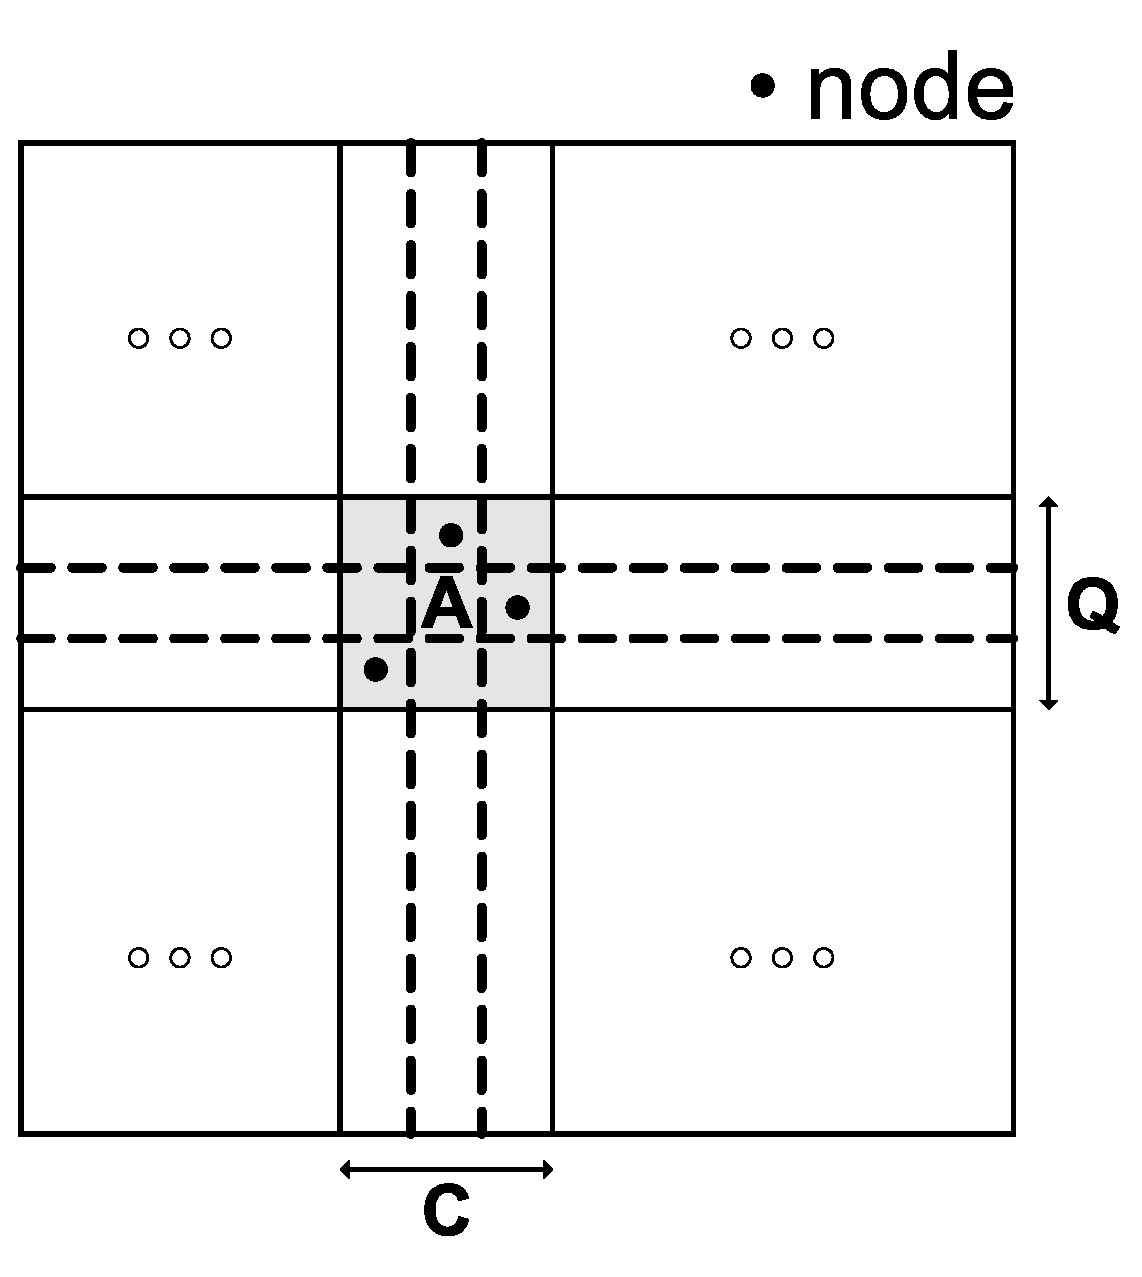
\includegraphics[width=1.8in]{space}
\caption{The caching and querying space.} \label{fig:space}
\end{figure}
\label{sec:table}
\begin{center}
\begin{figure*}[ht]
\centering
\begin{tabular}{c|c|c}
\begin{minipage}[t]{2in}
\centering
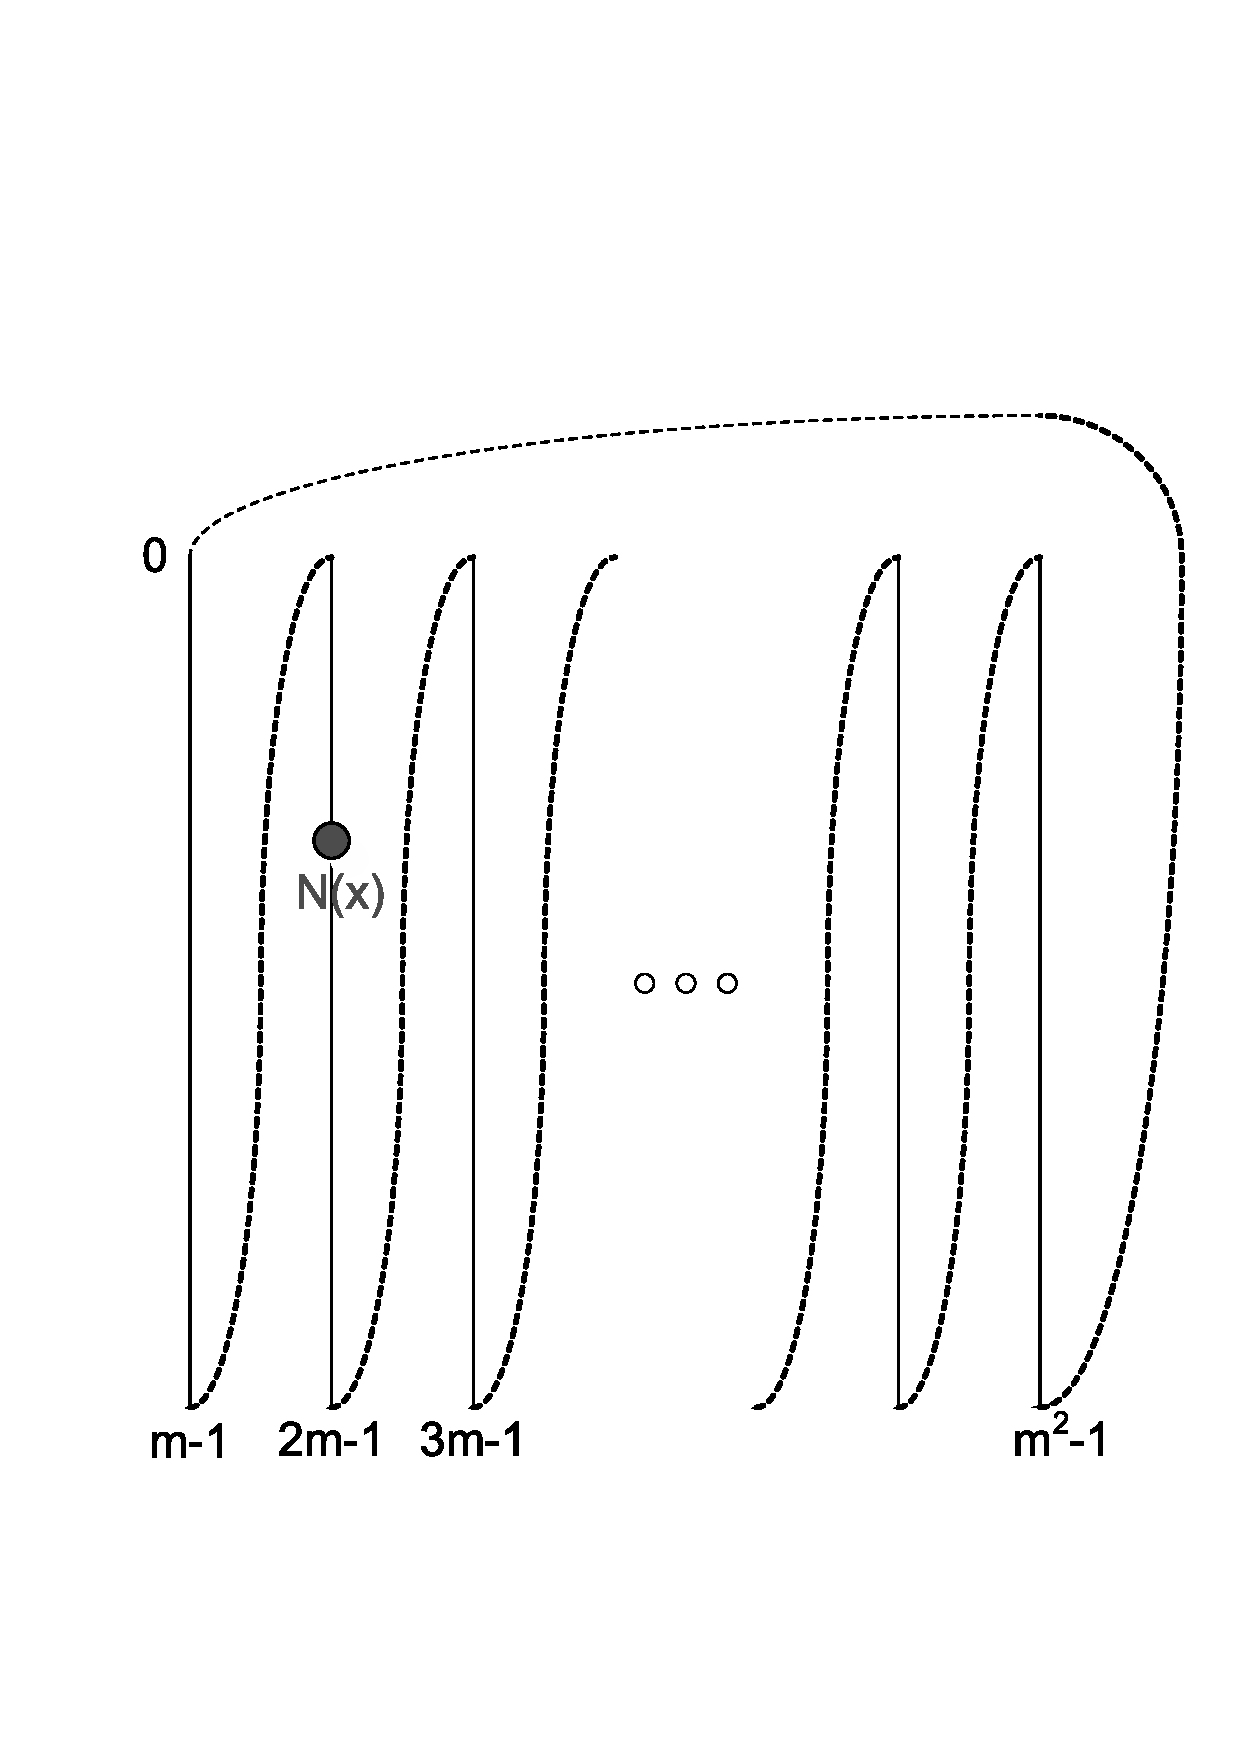
\includegraphics[width=1.5in]{cache}
\caption{Virtual ring 1 for caching.}
\label{fig:cache}
\end{minipage}
& \begin{minipage}[t]{2in}
\centering
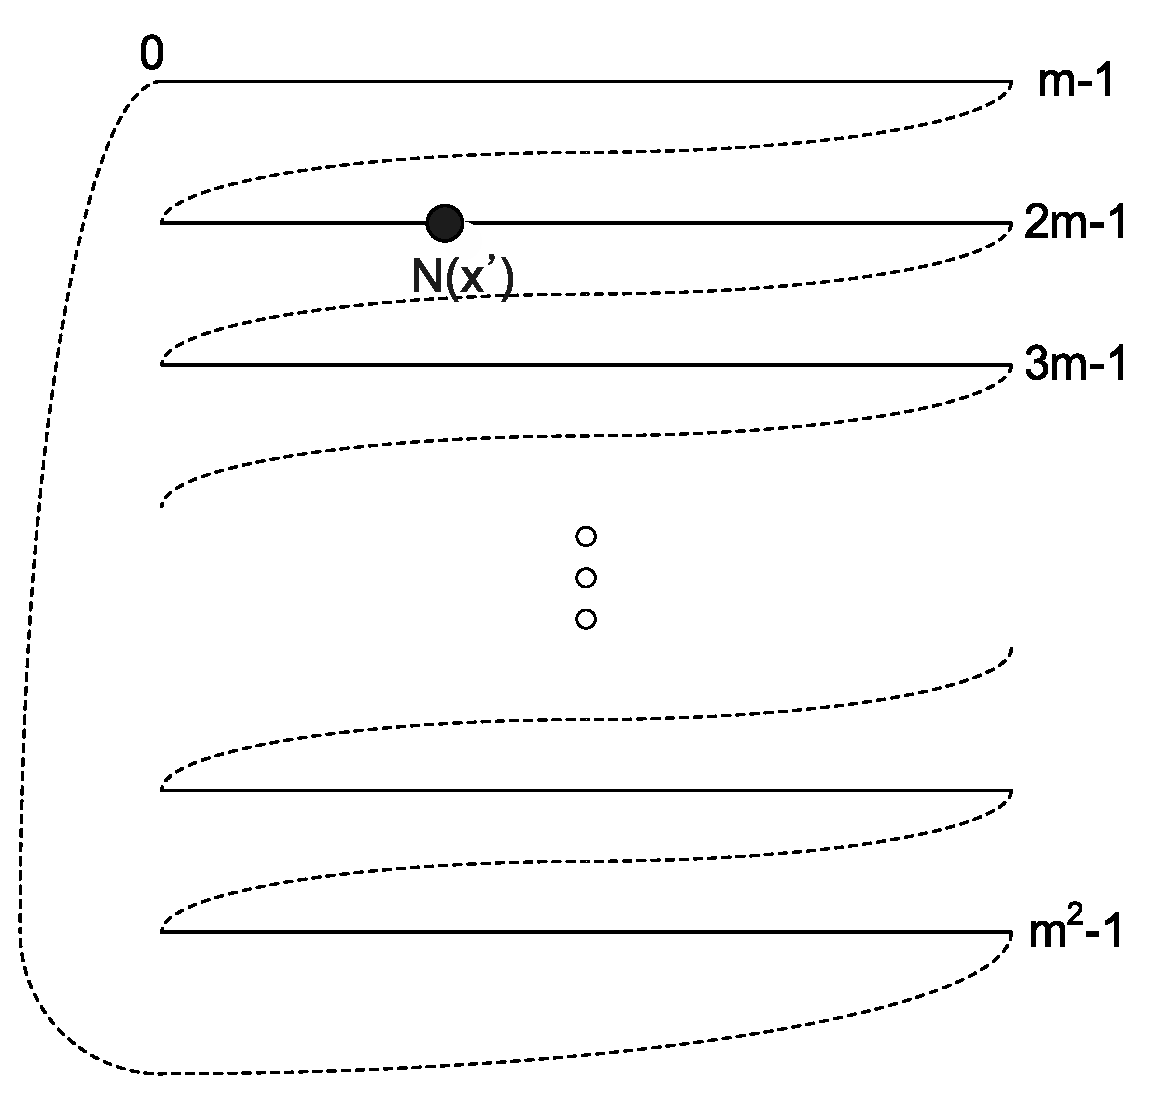
\includegraphics[width=1.5in]{query}
\caption{Virtual ring 2 for querying.} \label{fig:query}
\end{minipage}
& \begin{minipage}[t]{2in}
\centering
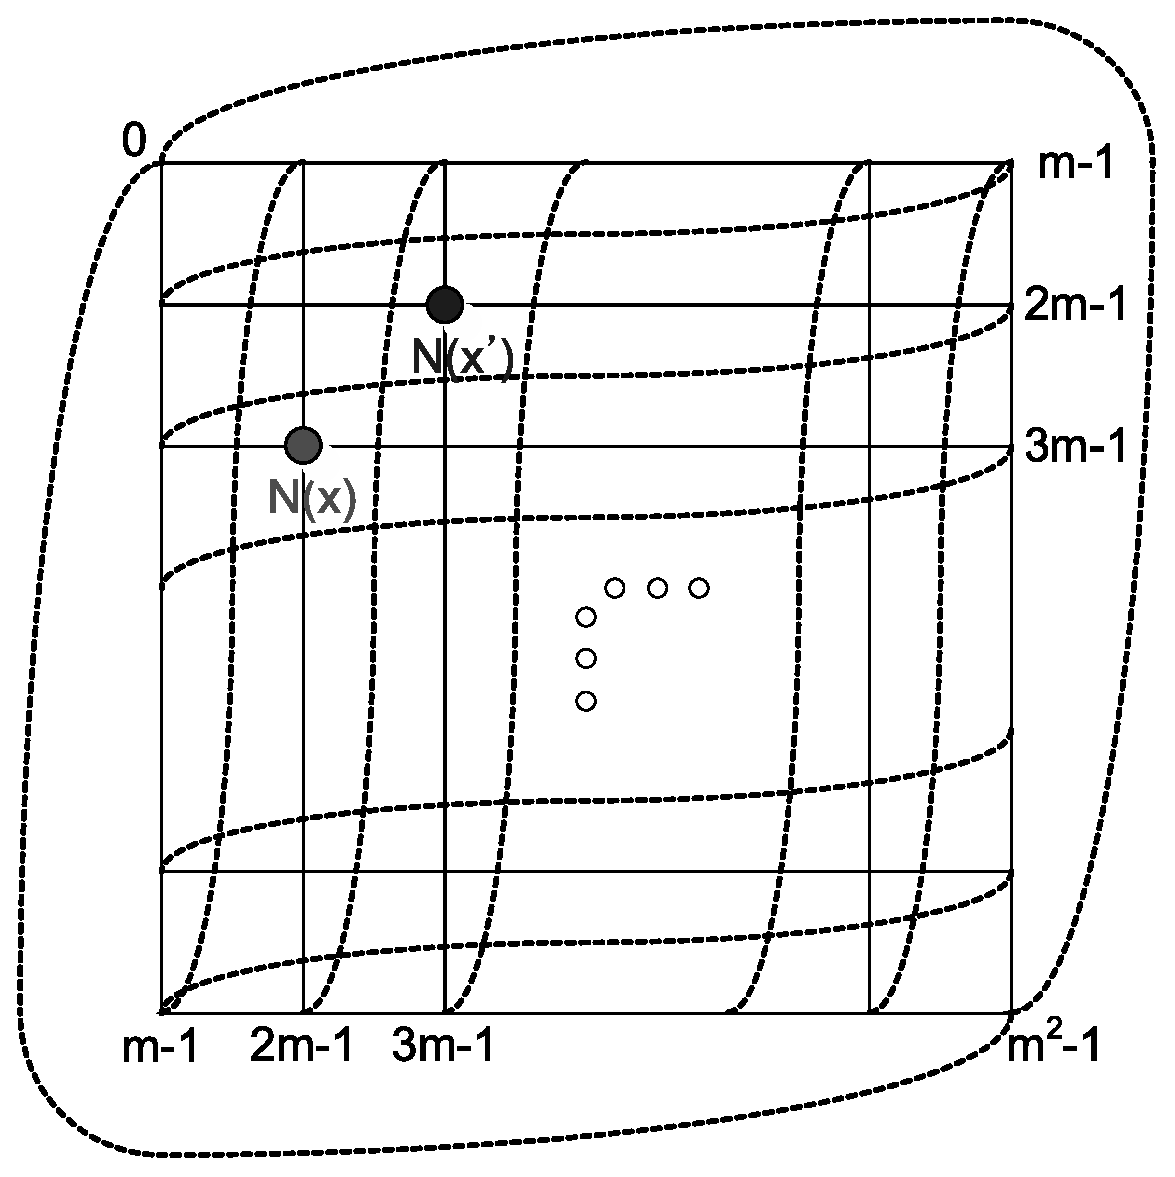
\includegraphics[width=1.5in]{combined}
\caption{The complete searching space.} \label{fig:combined}
\end{minipage}\\
\end{tabular}
\end{figure*}
\end{center}
\subsection{A Distributed unstructured table}
Our setting will be the standard P2P setting: there are $N$ nodes which can
communicate, store objects and perform queries.  In addition to nodes, there
are also bins.  Bins may or may not be occupied by a particular node.  The
number of bins is assumed to be fixed at some very large number, for instance
$2^{160}$.  The bins are arranged in a rectangular array, which in this work
we will assume to be square.  In the data structure of
Section \ref{sec:localtab}, each row and column intersect at exactly one
bin that may or may not be occupied by a node.  Instead of
querying and inserting along one row and one column, we will do so over a
sufficient number of rows and columns such that the probability of having 
more than one node in the overlapping set is very likely to be one.

Figure \ref{fig:space} depicts the 2-D array we use to cache (insert)
and query (search).  The area \textit{A} represents the
intersection of a particular cache and query operation.  We see in that
area, for example, there are three nodes, and so the query will be successful.  We need to
show several things to see that this algorithm will work in a distributed
setting: first show how to efficiently send cache and query messages to entire columns
and rows respectively; second show how to deal with nodes joining and leaving the network.

To deal with the above two problems we leverage existing work on building
routable 1-D P2P networks such as Chord\cite{is:Chord} and the small-world
model\cite{jk:Algorithmic}.  Rather than build a P2P network that is
explicitly two dimensional, we build two sub-graphs, each of which is a 1-D 
ring, which we can call the query ring and the cache ring.  Each P2P 
node has exactly one address, and hence position, on each ring.  This is
depicted in Figures \ref{fig:cache}, \ref{fig:query}, and \ref{fig:combined}; 
these drawings illustrate how  1-D rings for querying and caching 
locally overlay atop of the 2-D Deetoo array.
A node is located at $i$ with probability $c_{i}$ and a
query node is placed at location $j$ with probability $q_{j}$ in the query ring. 
$N(x)$ and $N(x^\prime)$ denote nodes whose addresses are $x$ and $x^\prime$, respectively.
$x^\prime$ is transposed address of $x$.

To create an ordering on the cache ring of increasing
along the columns and the query ring of increasing along the rows, the bin
address for a given node in the query ring must be the transpose of the
address on the cache ring.  
Assume that the size of the address space,
and hence number of bins, is $B=w^2$.
The address mapping algorithm is as
follows: Let $x$ denote an address on the cache ring. The address
$x$ can be expressed by
column element, $x_{i}$, and row element, $x_{j}$, such
that $x = w x_i + x_j$.
A translated address on the query ring $x^\prime$ is obtained by exchanging
column element and row element:
$x^\prime = w x_{j} +x_{i}$.

So, each P2P node then has two addresses in virtual 1-D rings and follows the usual
procedure for joining each of the two rings as described in \ref{sec:join}.
Notice that on the cache ring, the nodes in the same columns (and adjacent
columns) have adjacent addresses.  On the query ring, nodes in the same row
(and adjacent rows) have adjacent addresses.  Because the rings are efficiently
routable, it is also efficient to send a message to a randomly selected node near
the start of a column or row.  Similarly, to reach all elements of a row or
column, we can use a bounded broadcast on one of the two rings.  

\subsection{Bounded Broadcast}
\label{sec:broadcast}

In Deetoo, a bounded broadcast is accomplished with the following 
recursive algorithm:  
To broadcast a message over the region $[x, y]$, 
our routing algorithm finds any node in the given range firstly via greedy routing,
in which a node finds the closest node to the destination as its next node.
Let us assume that a node $x$ is the first node in the range recognized by greedy routing, 
then the message is sent to node $x$. 
Suppose $x$ has $F$ connections to nodes in the range $[x, y]$. 
We denote the $i^{th}$ such neighbor as $b_i$.
The node $x$ sends a bounded broadcast over a sub-range, 
$[b_i, b_{i+1})$, to $b_i$, except the final neighbor. 
Differently stated, $b_i$ is in charge of bounded-broadcasting 
in the sub-range $[b_i, b_{i+1})$. If there is no connection to a node in the sub-range, 
the recursion is ended and the node stays in the tree as a leaf node.
To the final
neighbor ($b_F$), $x$ sends a bounded broadcast in the range of $[b_F, y]$.
When a node receives a message to a range that contains its own address
the message is delivered to that node in addition to being routed to others.
Figure \ref{fig:tree} shows how this bounded broadcast forms a local 
tree recursively. The time required for this is $O(\log^2 N)$ as 
shown in Section \ref{sec:search_time}.

\begin{figure}
\centering
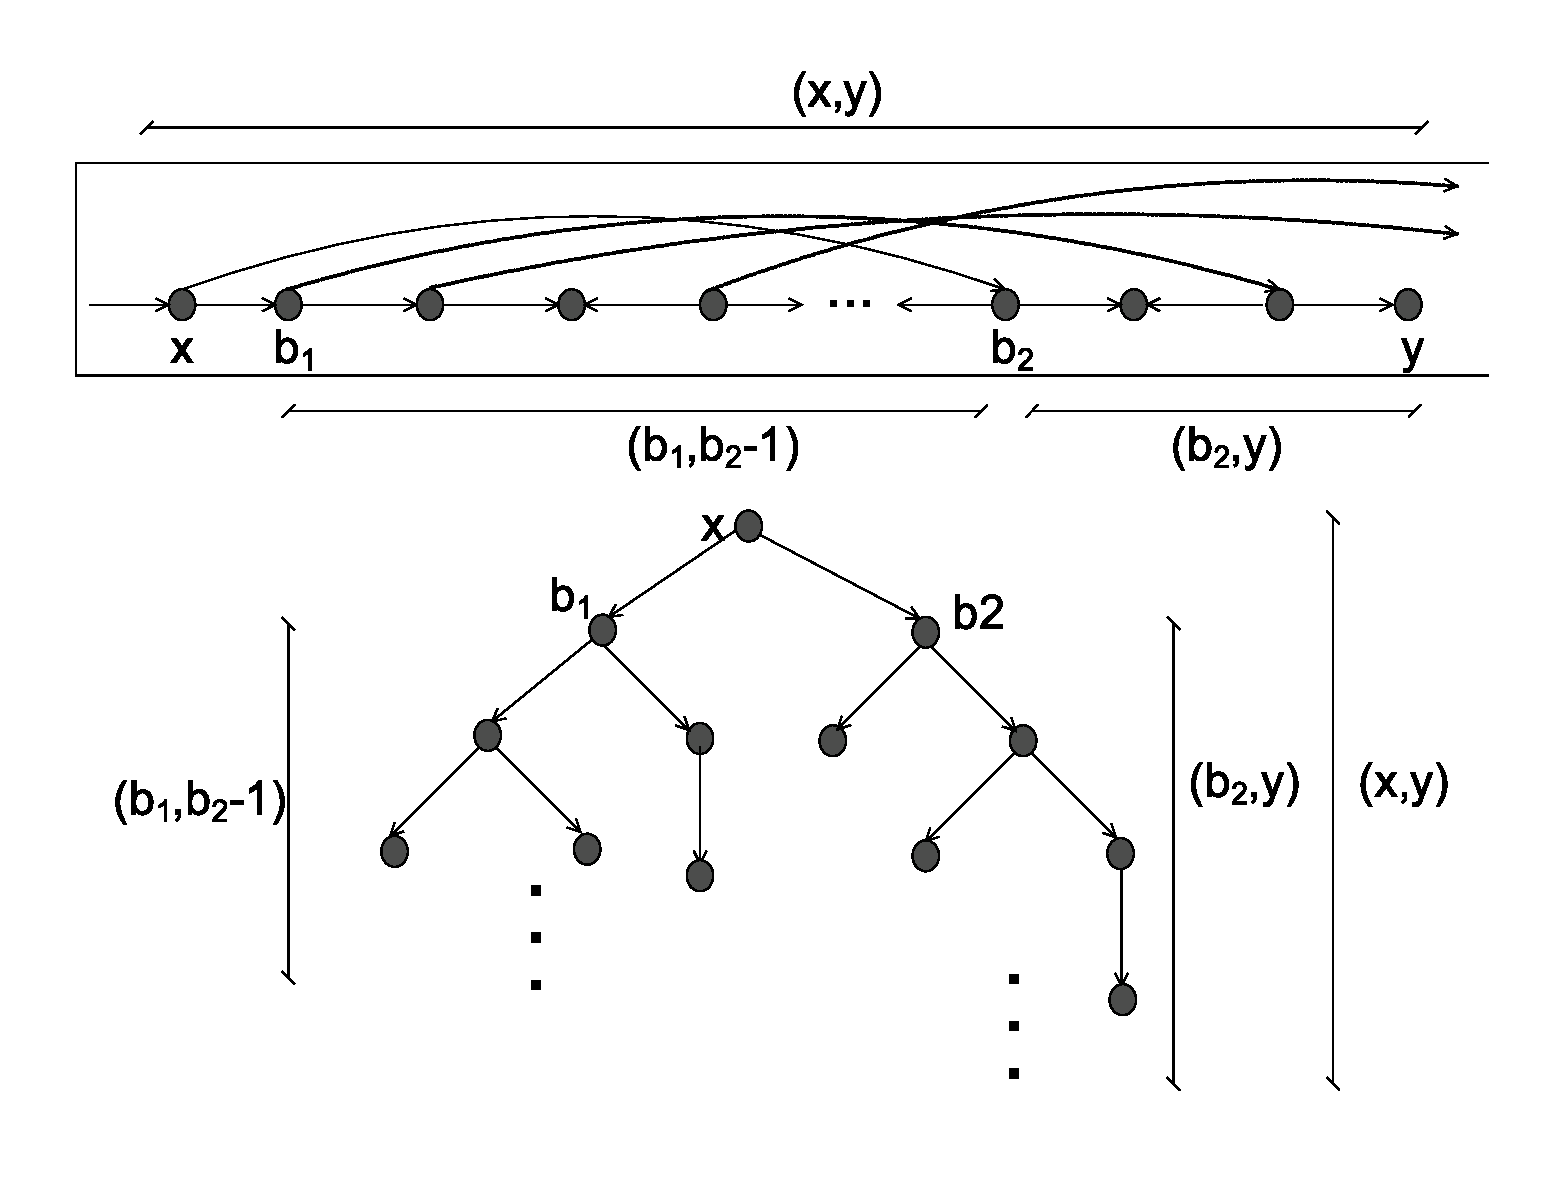
\includegraphics[width=2.5in]{tree}
\caption{Bounded Broadcast in range $[x, y]$} \label{fig:tree}
\end{figure}
\begin{center}
\begin{figure*}[ht] 
\centering
\begin{tabular}{c|c|c}
\begin{minipage}[t]{2in}
\centering
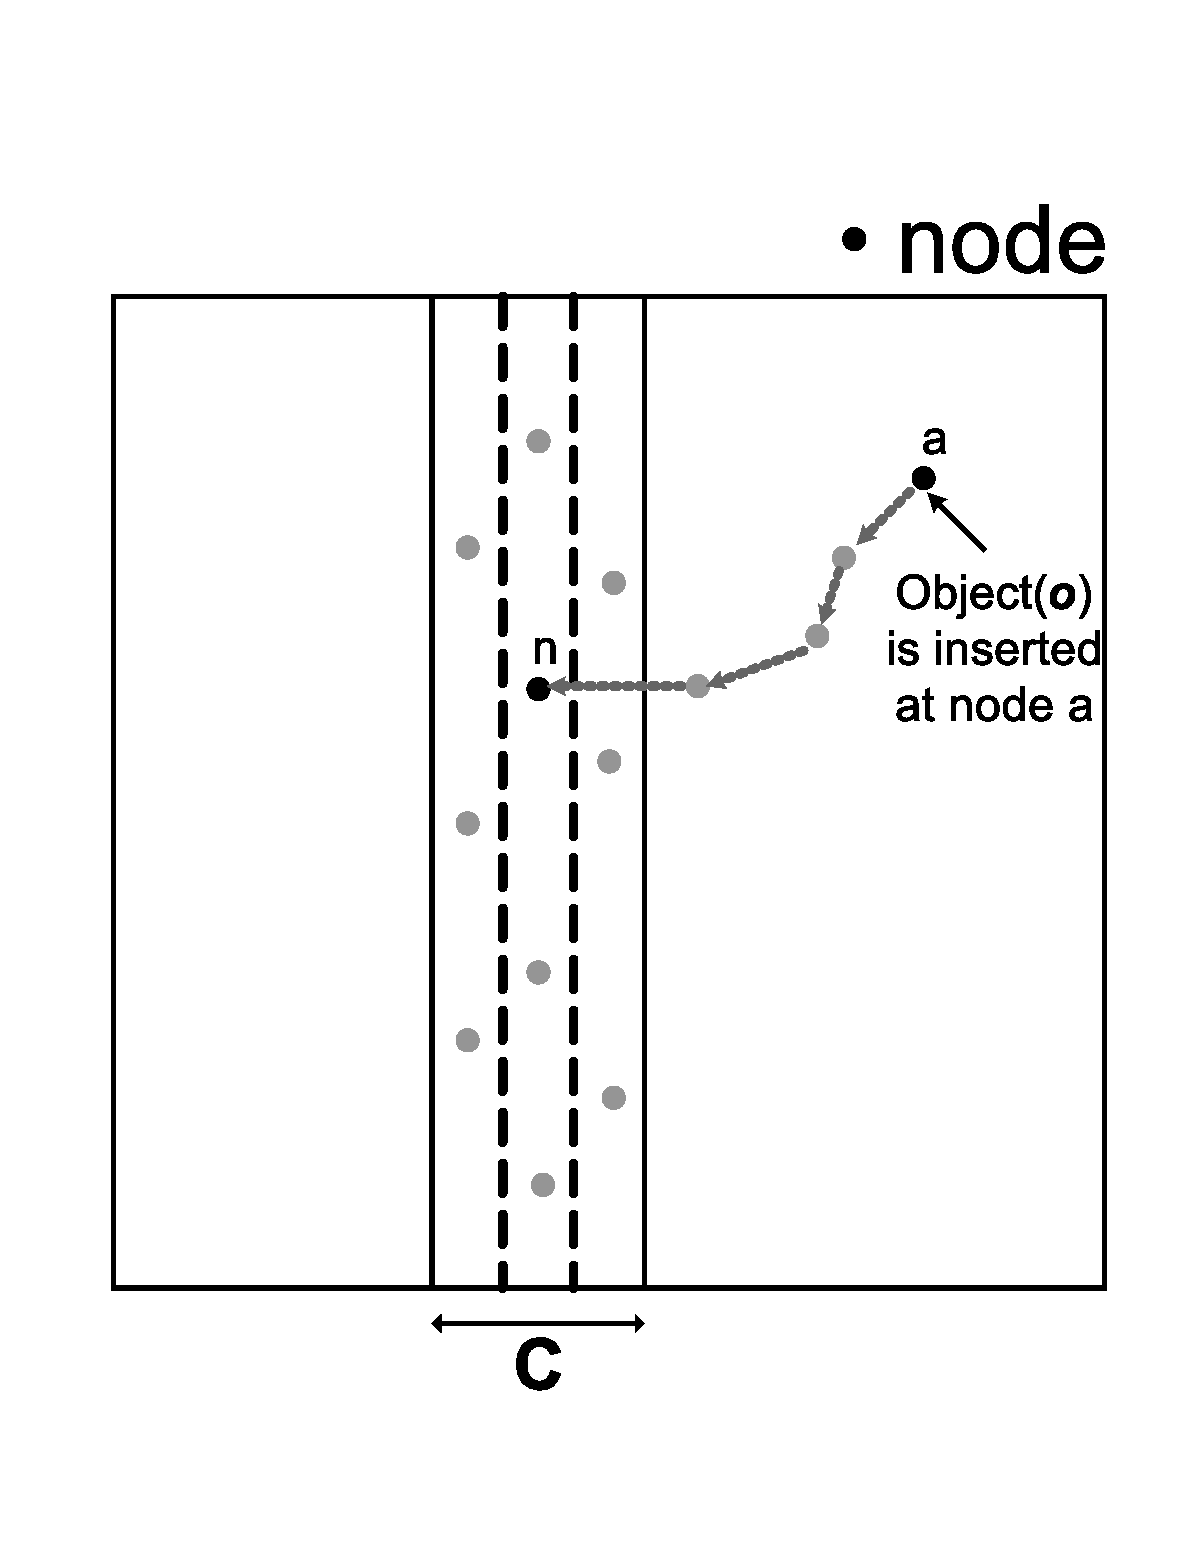
\includegraphics[width=1.4in]{cache_1}
\caption{An object(\textit{o}) is inserted at node \textit{a}. 
The message is routed to a node(\textit{n}) in the 
region for the bounded broadcast.}
\label{fig:cache1}
\end{minipage}
& \begin{minipage}[t]{2in}
\centering
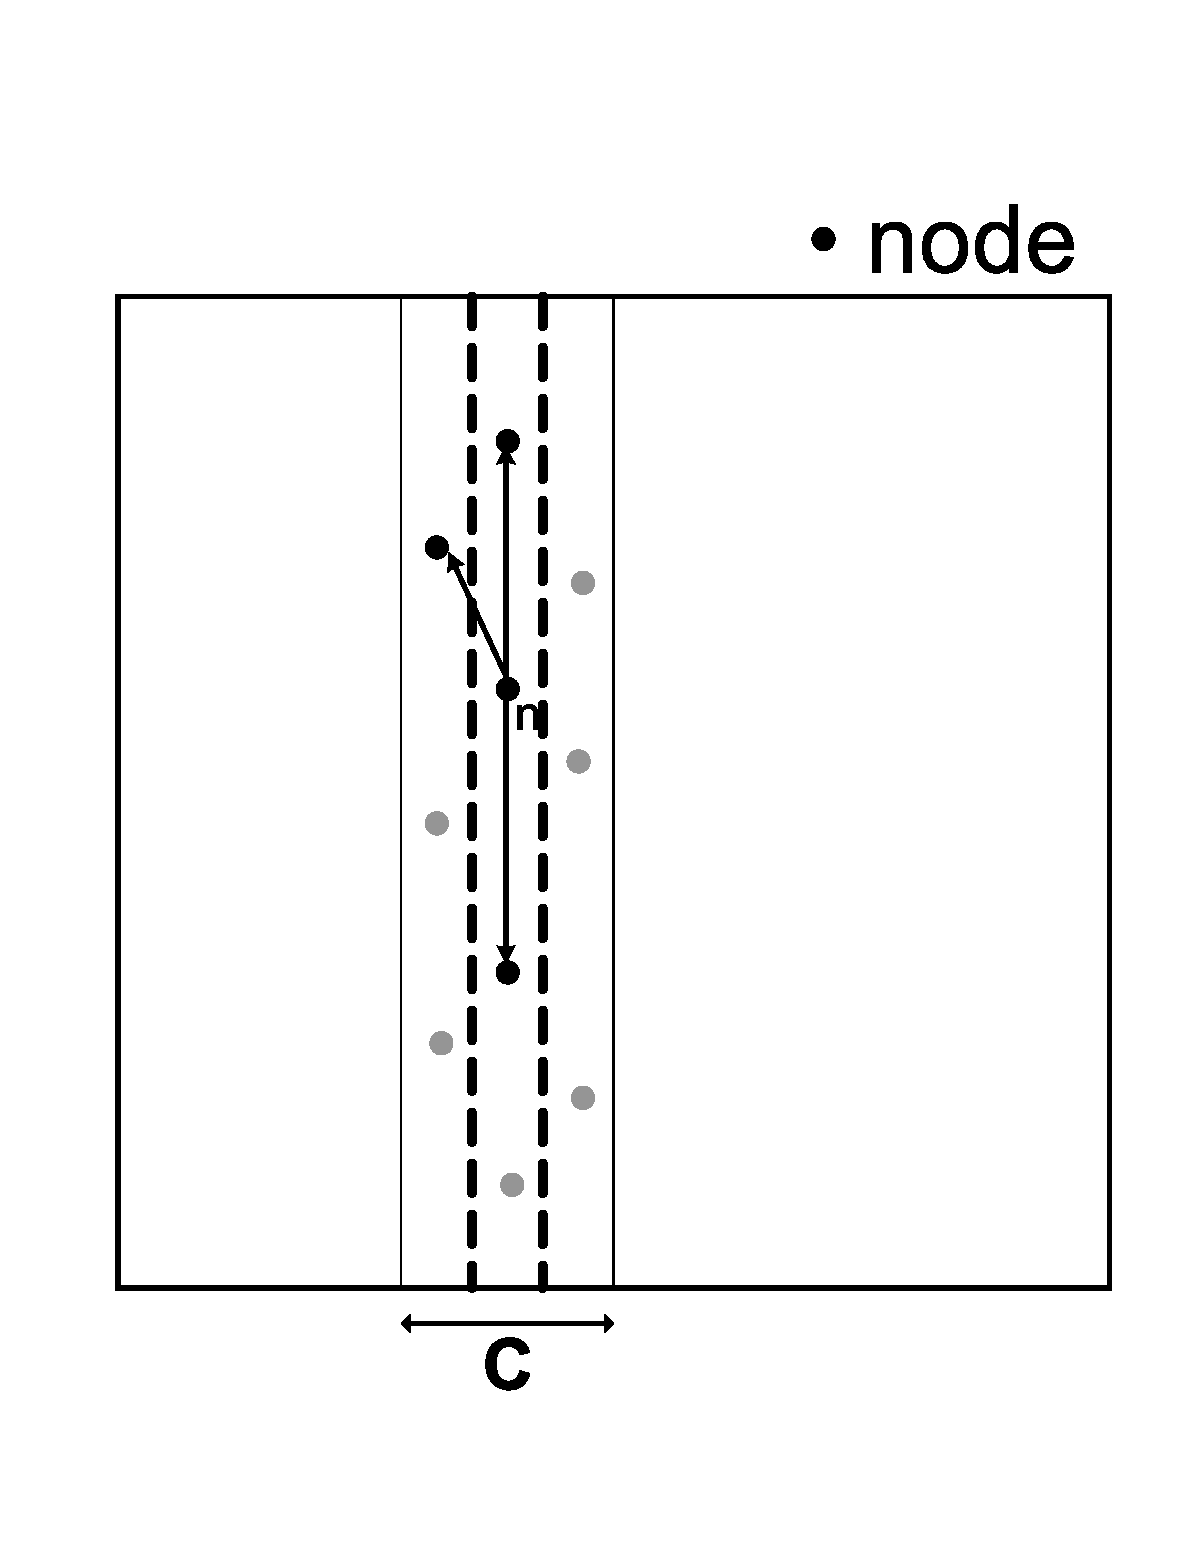
\includegraphics[width=1.4in]{cache_2}
\caption{The bounded broadcast starts at node \textit{n}.}
\label{fig:cache2}
\end{minipage}
& \begin{minipage}[t]{2in}
\centering
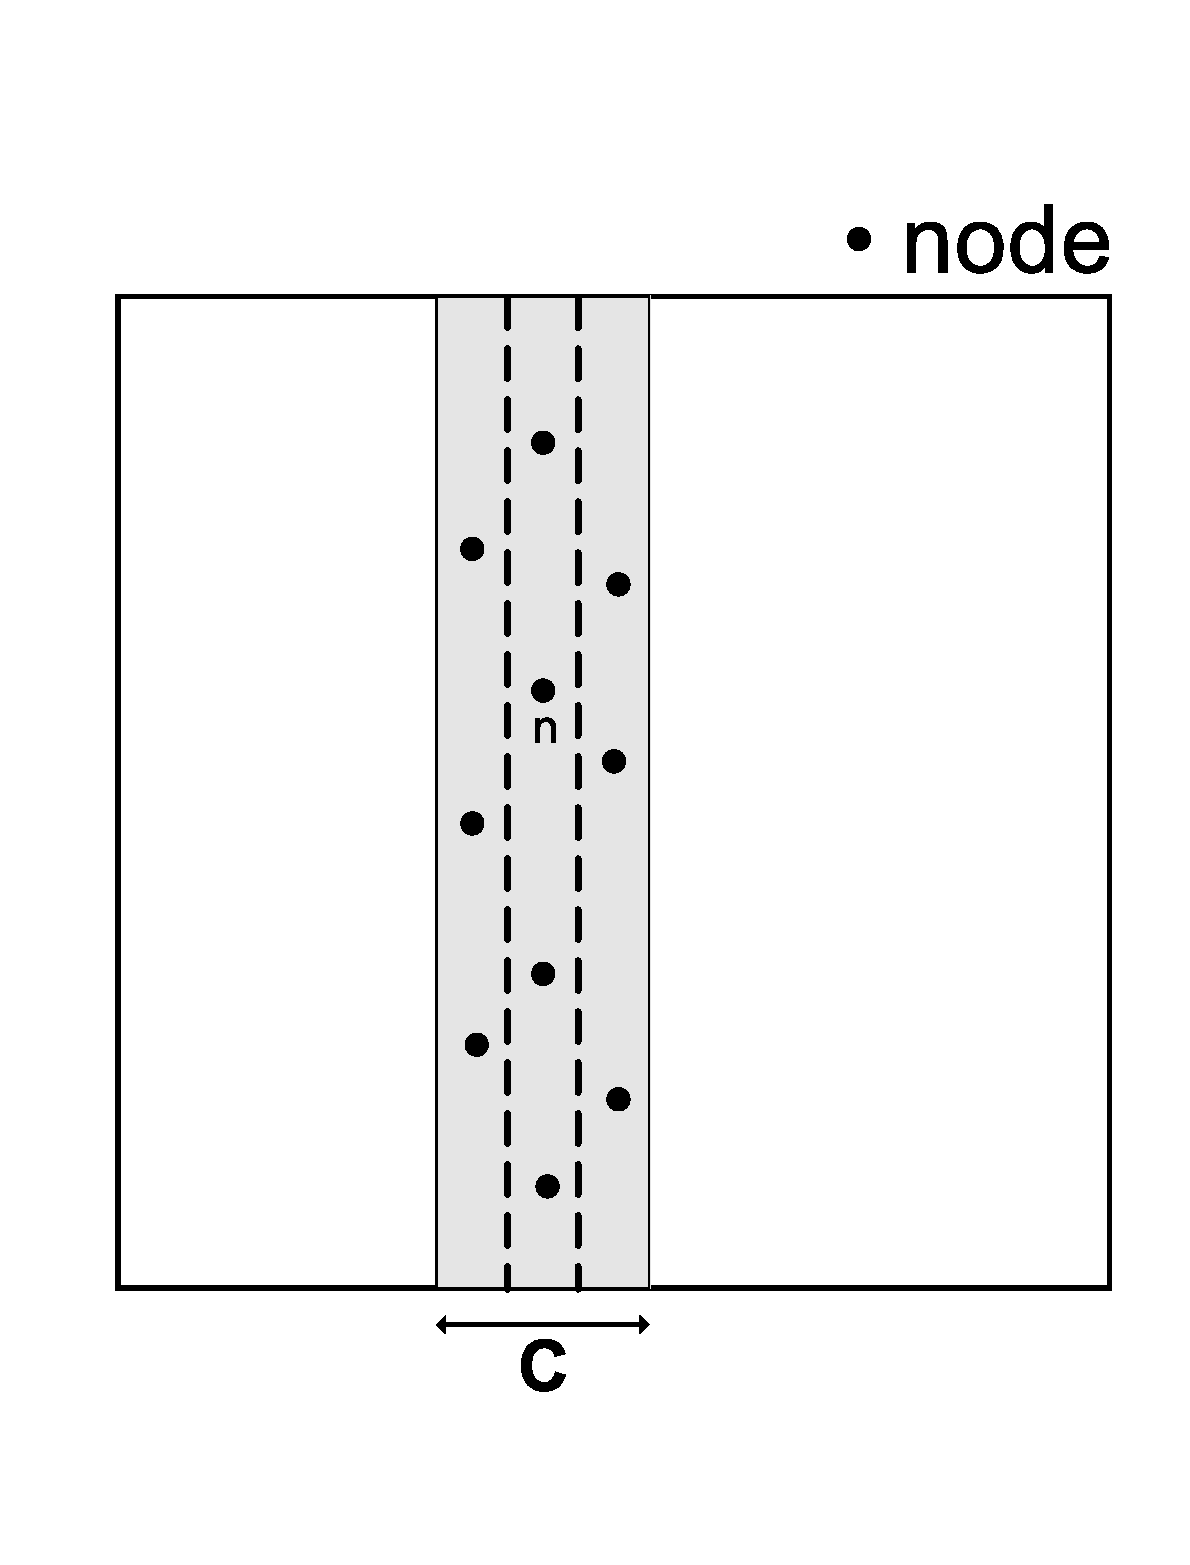
\includegraphics[width=1.4in]{cache_3}
\caption{All nodes in the range receive the message.} \label{fig:cache3}
\end{minipage}\\
\end{tabular}
\end{figure*}
\end{center}
\subsection{Data Insertion and Query}\label{sec:cache}
Deetoo is a search algorithm on a specific network structure. When an object
is inserted at a node $a$ as in Figure \ref{fig:cache1}, 
Deetoo selects, at random, a range for local broadcasting.
Node $a$ starts greedy routing to find a node 
$n$ in the range and $n$ starts bounded broadcasting 
within the range on the caching ring to replicate the object
(Figure \ref{fig:cache2}). 
%Bounded broadcasting size for caching ($C$) is given by
%$C=\sqrt{\alpha \frac{B}{N}}$, where $\alpha$ is a constant 
%\textit{replication factor} (this is derived in Section
%\ref{sec:analysis}).
All nodes in the range 
eventually receive a copy of an object, $o$ (Figure \ref{fig:cache3}).

Query resolution follows the same bounded broadcasting steps. The only
difference is that the query resolution is executed in the querying
space in which every node's address is transposed (stated  
in Section \ref{sec:table}) in
the caching space. 
%Bounded broadcasting size for a query, $Q$, follows the same formulation 
%as the caching size $C$ as shown above. 
Figures
\ref{fig:query1}, \ref{fig:query2}, and \ref{fig:query3} show the
steps involved in a query: node $a^\prime$ issues a query, node $n^\prime$ initiates a 
bounded broadcast, and node $n(o)$ resolves a query. Since all nodes in the area
\textit{A} have a copy of an object $o$, $a^\prime$ can retrieve
a desired object from any of the nodes in \textit{A}. By following these
steps, a query can be resolved if at least one node exists in
\textit{A}.
%Note that a user can select bounded broadcasting size by adjusting 
%$\alpha$. The bigger the $\alpha$, 
%the higher the probability to hit a node in \textit{A}, at the expense of 
%larger number of messages and replicas. 

%Users may want to insert objects into a network, or delete them from a network.
%The following explains how Deetoo manages both insertion and deletion.
%\begin{itemize}
%\item \textbf{Object Insertion: } When a new object is inserted to the network,
%copies of the object are created along some sets of columns in the matrix
%space (the number of columns is inversely proportional to the square-root
%of the network size) using bounded broadcasting. Unlike a DHT, each object does not have to have a
%unique identification number, and each inserted object does not have
%to map a key to the ``closest" node.

%\item \textbf{Object Deletion: }
%Objects do not stay forever in the networks.
When an object is obsolete, Deetoo provides a deletion that uses both 
caching and querying.
First, the deleter queries for an object which needs to be deleted.  Each
object is stored along with the original range into which it was inserted.
After the object's range is acquired, 
the \emph{deletion} message is broadcasted within the range in the same way the object
was replicated. As a result, Deetoo guarantees all replicated objects that are 
supposed to be stored in the nodes in the range to be removed.
%\item Join cost (show effetiveness of data insertion and deletion)
%\end{itemize}

\begin{center}
\begin{figure*}[ht]
\centering
\begin{tabular}{c|c|c}
\begin{minipage}[t]{2in}
\centering
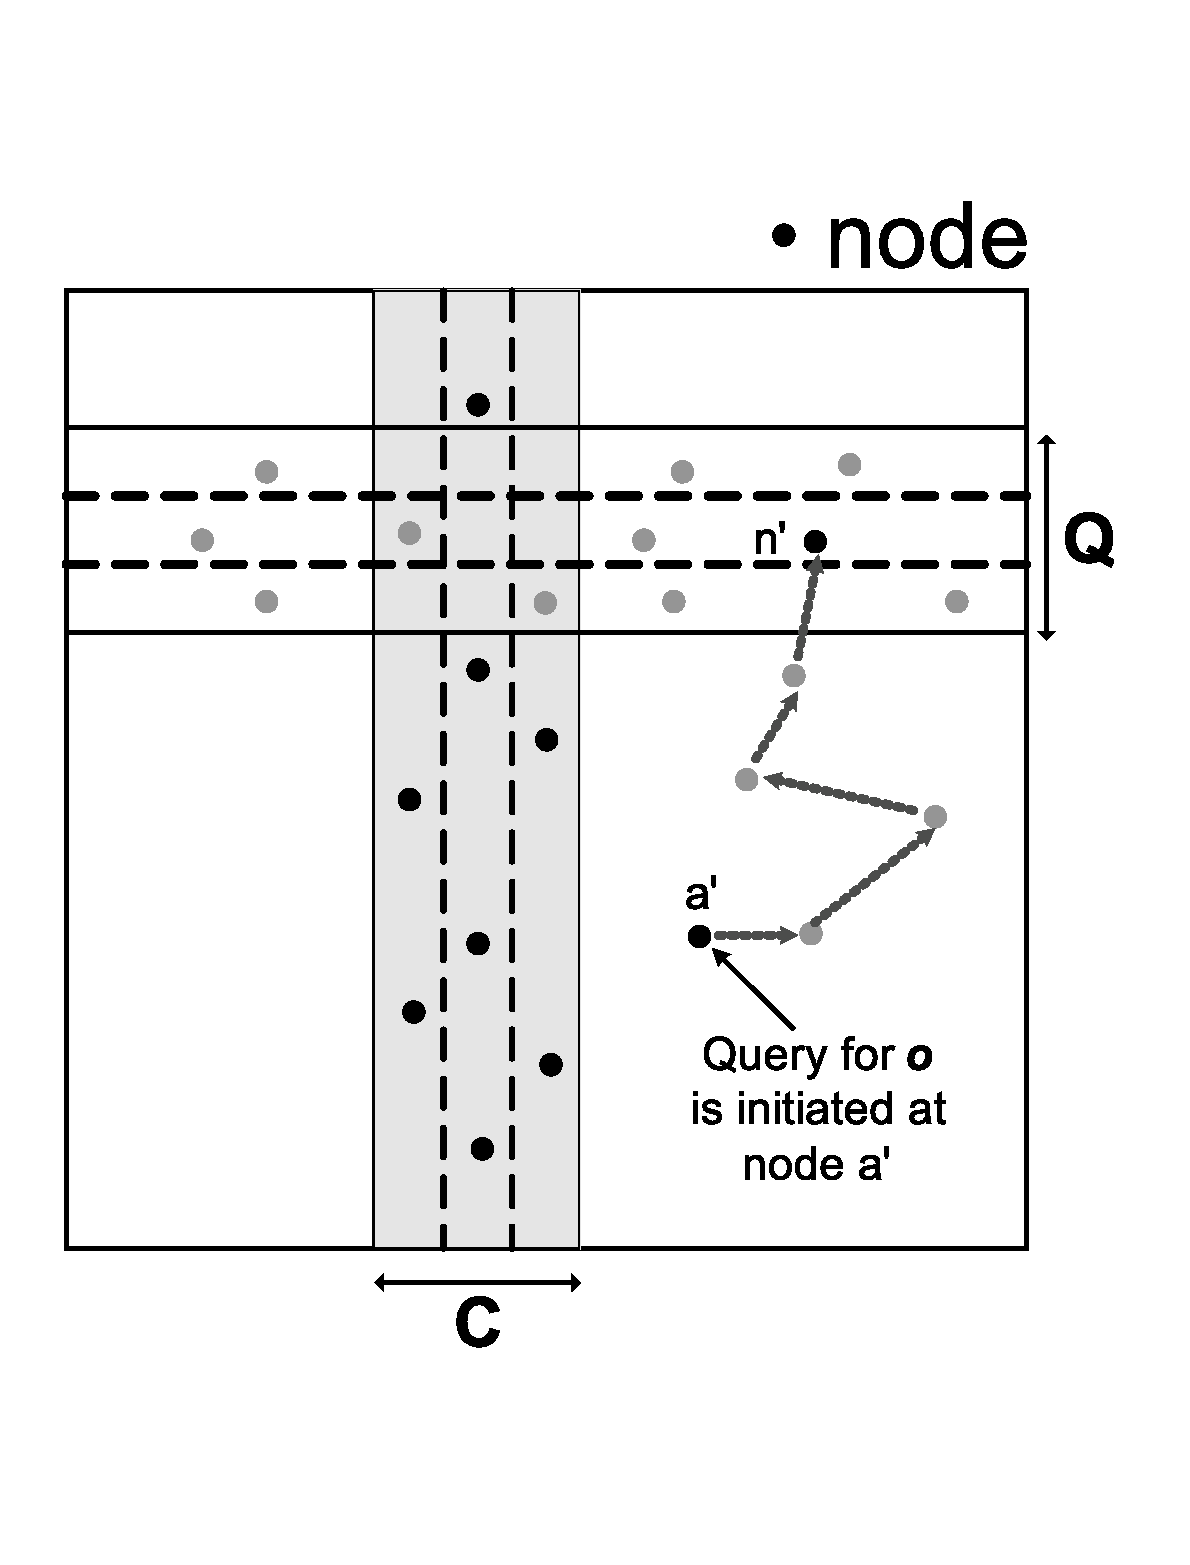
\includegraphics[width=1.4in]{query_1}
\caption{A query for object $o$ is initiated by a node
$a^\prime$.} \label{fig:query1}
\end{minipage}
& \begin{minipage}[t]{2in}
\centering
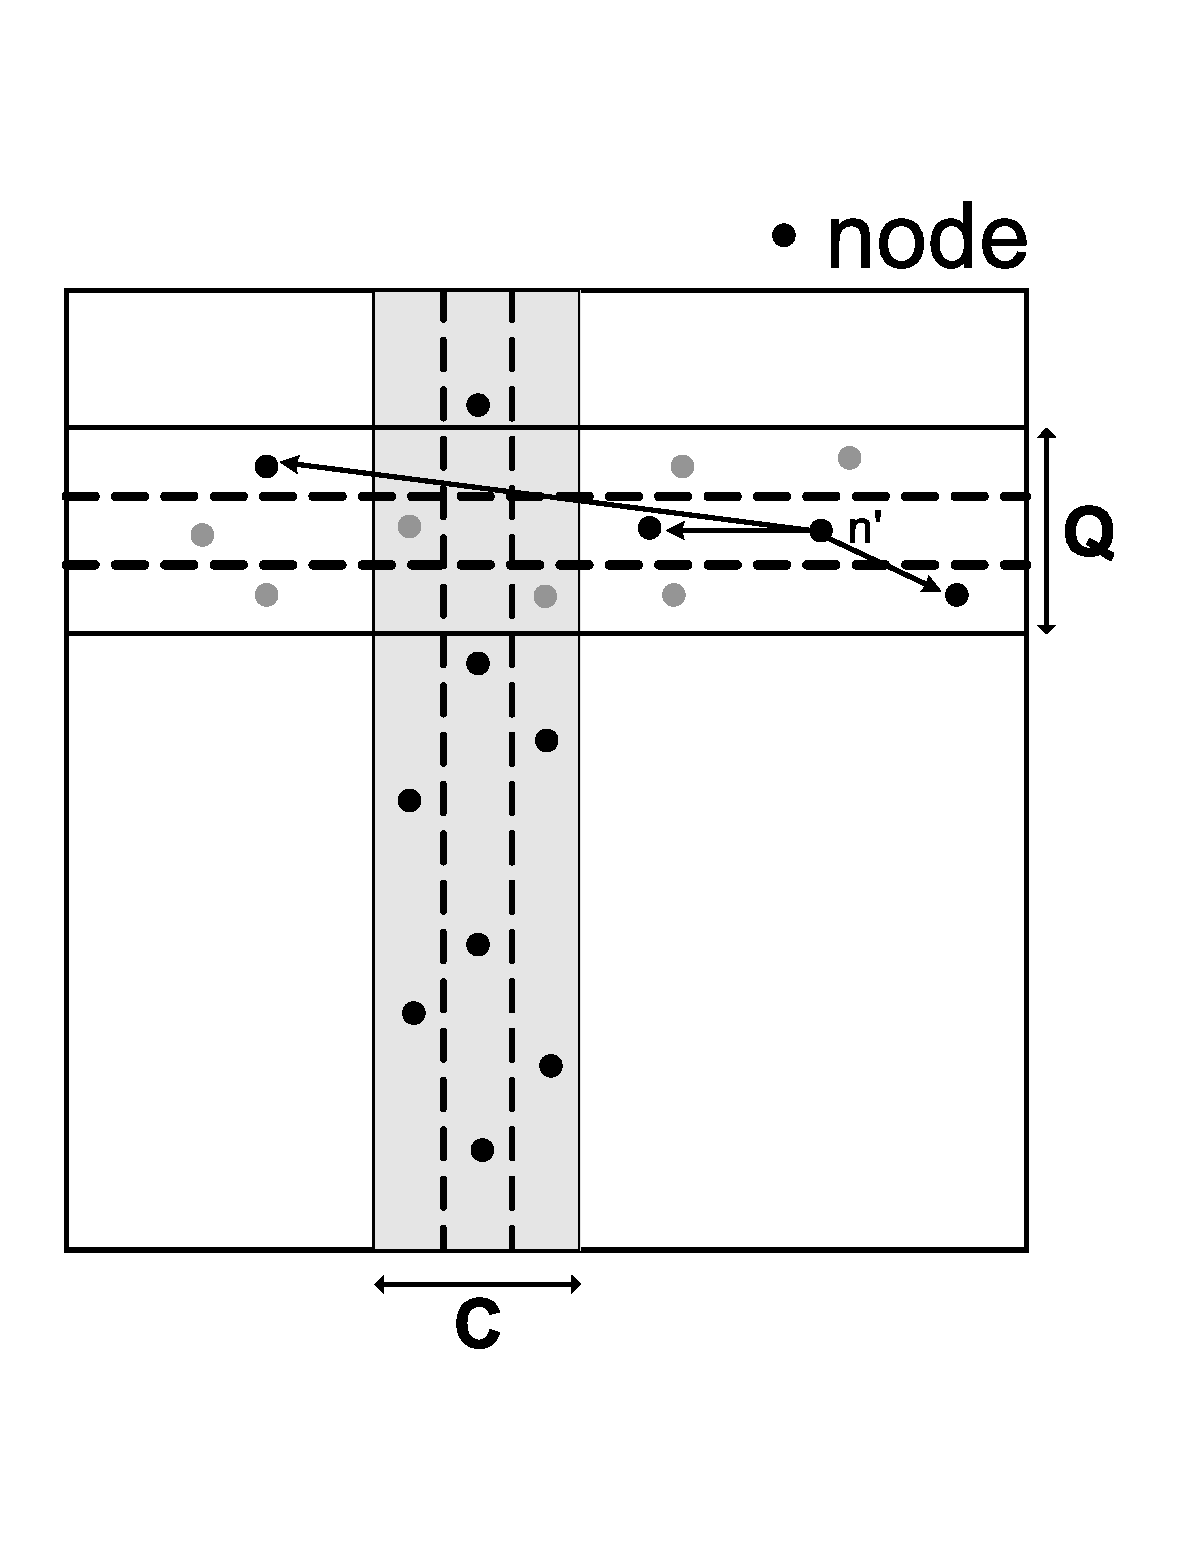
\includegraphics[width=1.4in]{query_2}
\caption{$n^\prime$ starts bounded broadcasting within $Q$}
\label{fig:query2}
\end{minipage}
& \begin{minipage}[t]{2in}
\centering
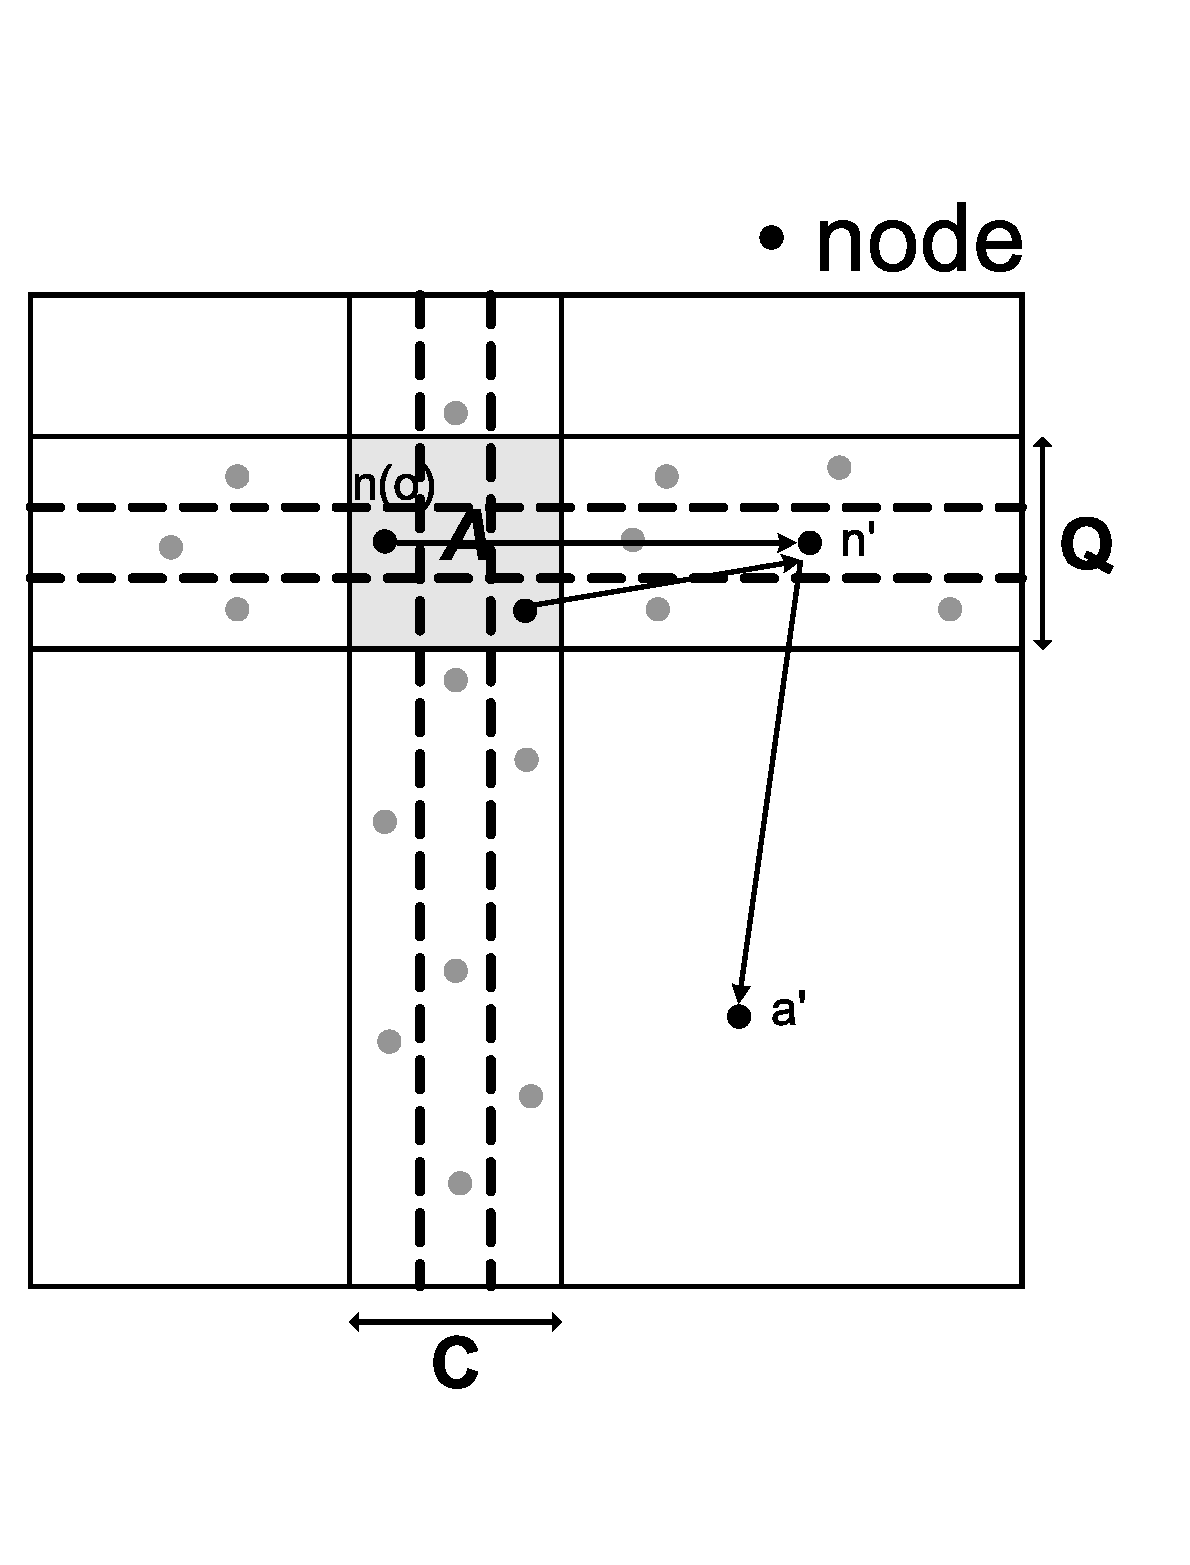
\includegraphics[width=1.4in]{query_31}
\caption{Finally, $a^\prime$ retrieves an object from a node $n(o)$.}
\label{fig:query3}
\end{minipage}\\
\end{tabular}
\end{figure*}
\end{center}

\subsection{Node Joins, Leaves, and Stabilization}\label{sec:join}
Deetoo requires that each data object is replicated over the desired 
range in a network. However, a new node joins the network with no replicated 
objects. 
We want a constant success probability regardless of node joining or leaving.
Since objects should appear on all nodes for the range into which they were
inserted, it is necessary to replicate objects when a new node joins.
Deetoo relies on a new node copying objects from its new neighbors. 
We define this replicating process as \emph{stabilization} in this paper.

When a new node joins a network, the following steps are taken:
A new node picks a random address, then it makes a connection to two adjacent
neighbors and one short-cut neighbor based on Kleinberg's
\emph{inverse $r^{th}$-power distribution}. As a final step, it copies objects 
from a neighbor in the same column in matrix space.
%\begin{enumerate}
%\item select two different random addresses, 
%\item calculate minimum ring distances to neighboring nodes which have 
%      left closest address and right closest address,
%\item find a proper place on the virtual ring space by selecting address 
%      whose minimum distance to neighbor node is bigger than the other,
%\item pick a random address
%\item obtain an address and 
%\item makes a connection to two adjacent
%      neighbors and one short-cut neighbor based on Kleinberg's
%      \emph{inverse $r^{th}$-power distribution}, 
%\item as a final step, copy objects from neighbors in the same 
%      set of sub-rings (in the same columns in matrix space). 
%\end{enumerate}
%\begin{figure}
%\centering
%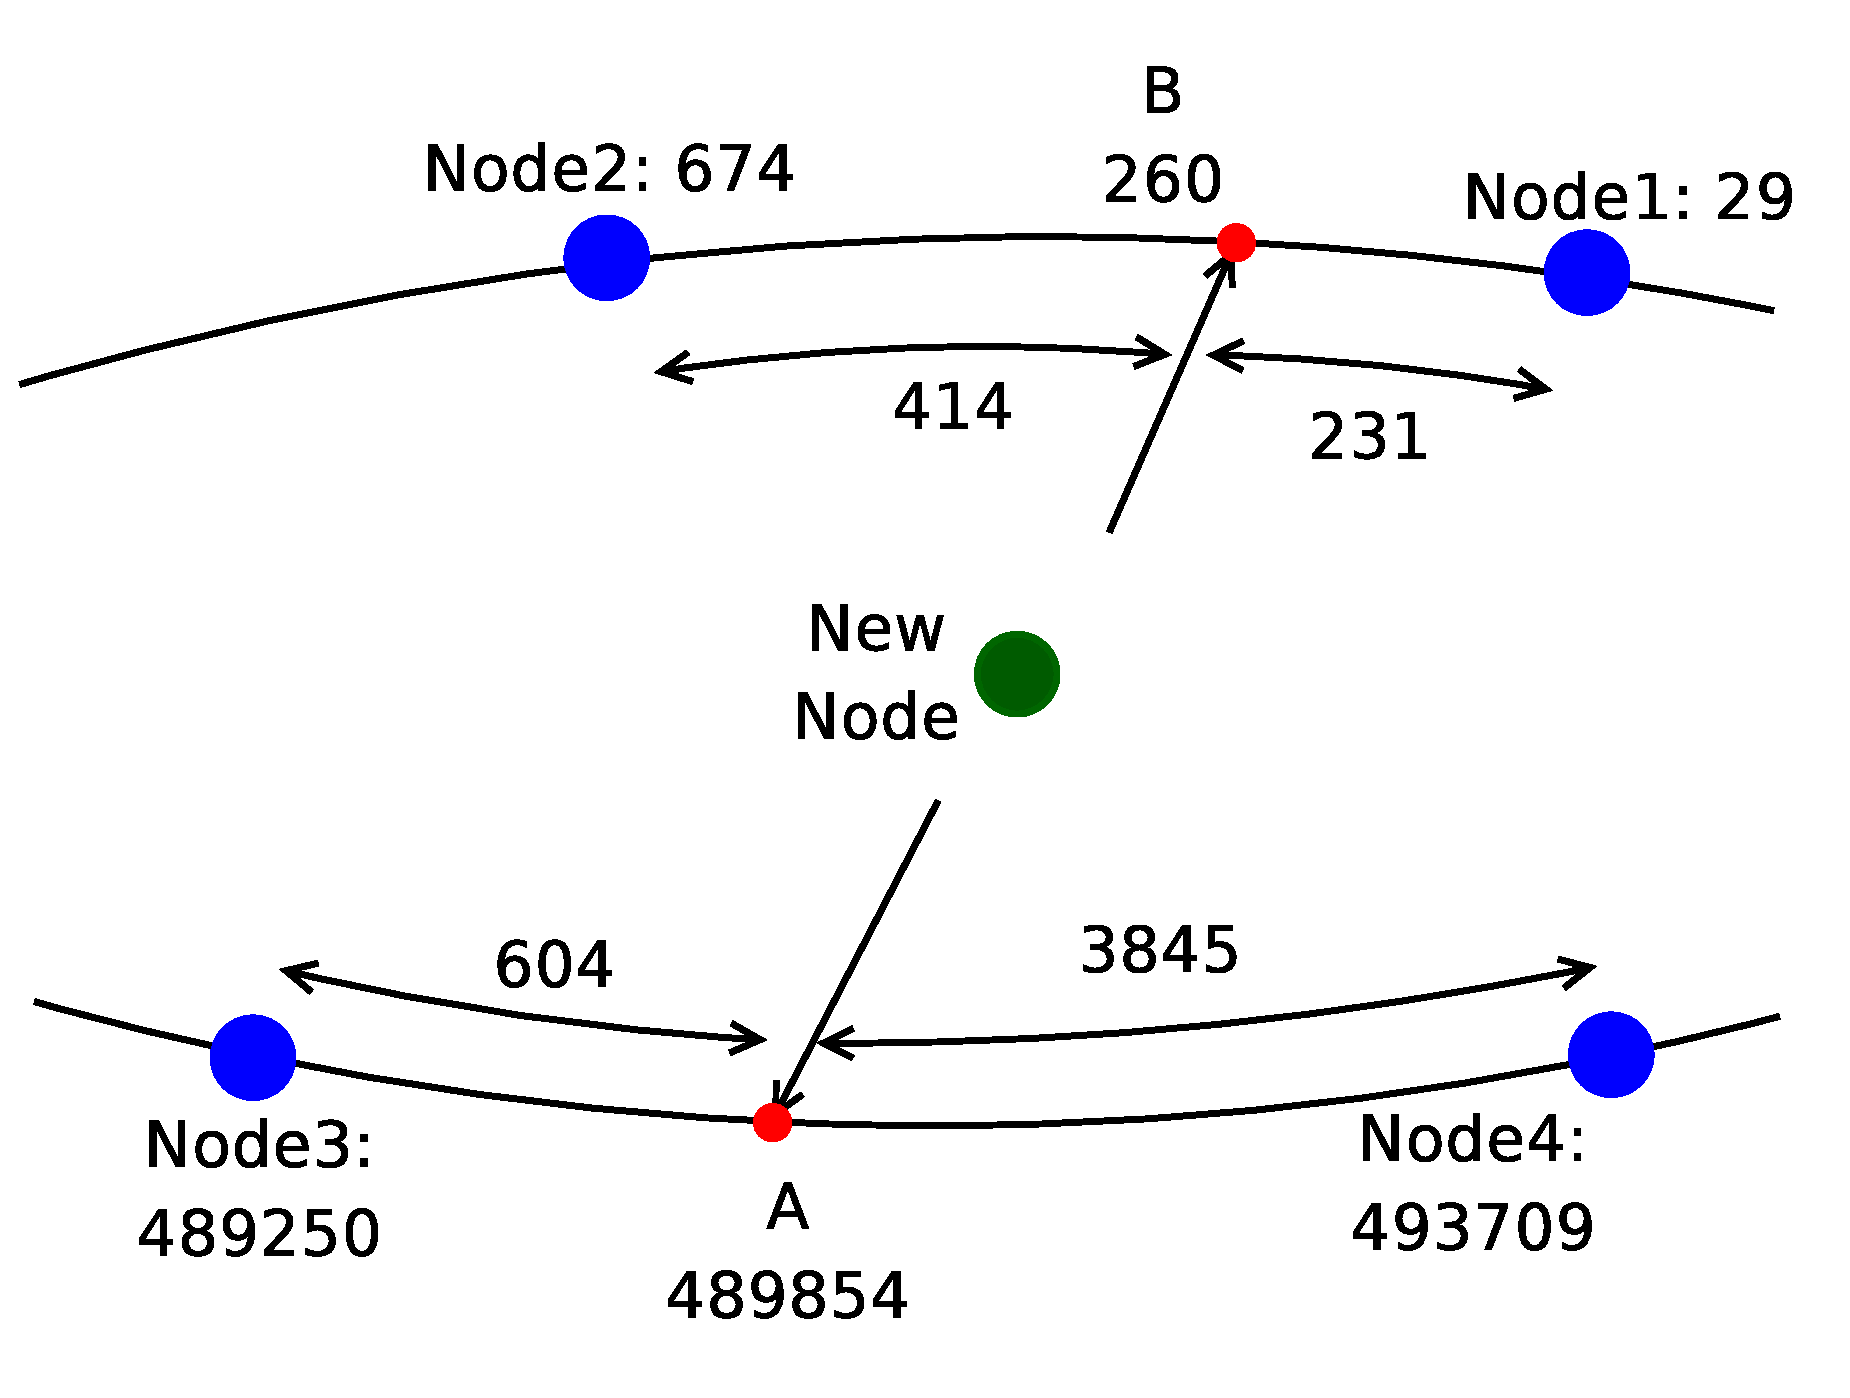
\includegraphics[width=3 in]{evenNet}
%\caption{Choosing a position on the ring when a node joins Deetoo.} \label{fig:join}
%\end{figure}
%Figure \ref{fig:join} shows how a new node finds its right place.
%From randomly selected positions \emph{A} and \emph{B}, the nearest neighbors are 
%\emph{node1} and \emph{node3}. Between these two nodes, 
%\emph{node3} has a bigger distance to \emph{A} than the distance 
%from \emph{node1} to \emph {B}. Thus, a new node takes a position \emph{A} as 
%its new address. 
\iffalse
%redundant with the above
Each object must keep its range information as well as the object itself where 
it was initially inserted to the network so that as nodes join and
leave the objects can be maintained on their randomly selected column.
% above sentence may need to be modified.
After a node obtains a proper address, the node sends requests to 
its newly connected neighbors in order to replicate objects.  
\emph{Stabilization} plays a role in this stage of replication. 
The following describes how all objects in the same boundary are 
copied to the new node from neighbors: 1) The new node retrieves the object's range
from the neighbor's object list. 2) The range is recalculated with a given 
replication factor. 3) It copies the object from the neighbor only if its address
lies on the recalculated range. 4) The processes 1) through 3) is repeated 
for all objects from both adjacent neighbors.
%\begin{enumerate}
%\item Retrieve the object's range from the neighbor's object list.
%\item Recalculate range with a given replication factor.
%\item Copy the object from the neighbor only if the new node's address 
%lies on the recalculated range.
%\item Repeat 1 through 3 for all objects from both adjacent neighbors.
%\end{enumerate}
If we assume that there exist \emph{k} unique objects in the network whose size is \emph{N}, 
each node maintains $k\frac{\alpha}{\sqrt{N}}$ objects on average, where $\alpha$ is a 
replication factor. In the stage of stabilization, the node is able to receive objects 
from both neighbors. The maximum number of objects which need to be transferred is limited to 
$O(\frac{1}{\sqrt{N}})$.
\fi
We analyze \emph{stabilization cost} in Section \ref{sec:stabilization_cost}. 
We also simulate stabilization cost at the time of new node joins 
under churn and compare the simulation result with an analytical model.  
The simulation result shows that Deetoo requires very low stabilization cost. 
When a node leaves or fails, our protocol
does not need to do anything because all objects have already been copied to
all nodes in the same set of columns. Thus, neighbor nodes keep exactly
the copies of the objects held by leaving or failing nodes.

\section{Analysis of Deetoo}\label{sec:analysis}
Our analysis focuses on the probability of a query being successfully resolved
($P_{s}$), the communication cost ($K$), and the search time ($T$),
to show that the Deetoo protocol for unstructured P2P
networks is efficient and scalable. We assume that
address space ($B$) is fixed as $B=m$ $\times$
$m$. Additionally, the caching probability we
cache at $i$, $c_{i}$, and the querying
probability we put a query at $j$, $q_{j}$, are both
uniformly distributed. 
%Third, the caching and querying probability are the same at any location. 
Finally, at most one node per
a bin in matrix space is allowed for all nodes to have a unique
address.
%Our analysis and simulation about search hit consider only 
%exact matching search. 


\subsection{Success Probability}
\label{sec:suc_prob}
In Deetoo, queries are unstructured and load-balanced, which means
that the probability that a given node receives a query is independent
of the query and equal for all nodes.
%One column or row has an address space of length of $\sqrt{B}$. 
For each object and query pair, there
is a region of size $A$ in the grid address space that receives both the query
and the cache. The only way the query will not be resolved is that the region
has no nodes.  Since every configuration of $N$ nodes in the address
space of size $B$ is equally likely, the probability there is a miss is given
by $P_{miss}=\frac{{{B-A}\choose N }}{{B \choose N}}$.

When $N+A\ge B$, the above is fairly trivial to evaluate, but we are
interested in the sparse case when $N+A<B$, which is to say the query/cache
overlap region and the number of nodes are both small compared to the total
number of bins.  Define $E=B-N-A>1$, which can be thought of as the number of
empty bins in the case of a miss.
Using Sterling-type bounds on the factorial, one directly obtains:
$P_{miss} < e^{-\frac{AN}{B}}\sqrt{1+\frac{AN}{BE}}e^{\frac{1}{12E+1}}$.
Thus if we set $C$ and $Q$ such that
$CQ=A=\alpha B/N$, we have
$P_{miss} < e^{-\alpha}\sqrt{1+\alpha/E}e^{\frac{1}{12E+1}}$.
One can find a similar lower bound that shows that
$P_{miss}/(1-\alpha)\rightarrow 1$ as $\alpha\rightarrow 0$.
If $AN$ goes to zero as $N$ gets large, $P_{miss}\rightarrow 1$,
and this result can be extended to any system with independent queries and
caching and where each node is equally likely to be used for each query or
cache, hence Deetoo is optimal in terms of the asymptotic of query/cache cost
trade-off.
The derivation of these results is omitted due to
lack of space.
When $E$ is large, as is the case for large networks with large address
spaces and non-negligible caching, $P_{miss}\approx e^{-\alpha}$.
So, we are able to have success probability solely as a function of the 
constant replication factor $\alpha$, and 
independent of the number of the nodes.

\subsection{Communication cost}
In order to check the network's scalability, communication costs
are examined in this section. Each caching message is transferred to all the
nodes in the shaded area in Figure \ref{fig:cache3}, and this area has
$C\sqrt{B}$ bins. By default, we set cache and query ranges are equally.
The expected number of nodes per bin is $p=N/B$.
From the previous section we see
$C = Q = \sqrt{\alpha B/N}$; therefore the expect caching cost or querying
cost $\langle K\rangle$ is:
\begin{equation*}\label{th}
\langle K\rangle = pC\sqrt{B} = \frac{N}{B}C\sqrt{B} = \frac{N}{B}\sqrt{\frac{\alpha B}{N}}\sqrt{B}
= \sqrt{\alpha N}
\end{equation*}
One can show that $K$ is distributed almost as a Poisson distribution, and
therefore the fluctuations in $K$ are not very large.  This proof is omitted
due to lack of space.
From the above analysis, we show that a query or a caching of an object in the network
generates $O(\sqrt{N})$ messages.

\subsection{Search time}
\label{sec:search_time}
Search time can be analyzed by computing the average
depth of the tree formed by the bounded broadcast presented in
Section \ref{sec:broadcast}. When we assume that each node 
has a connection to its nearest neighbors on both rings as well as
one shortcut connection to a node at distance $d$ with probability
proportional to $1/d$, we can show that the expected depth of the 
tree is $O(\log^2 N)$. 
Our proof is analogous to computing the average time 
to reach a node using greedy routing as in \cite{jk:Information,
pr:Symphony}, while search time of 
Deetoo measures the average maximum depth of the local trees.
\begin{figure}
\centering
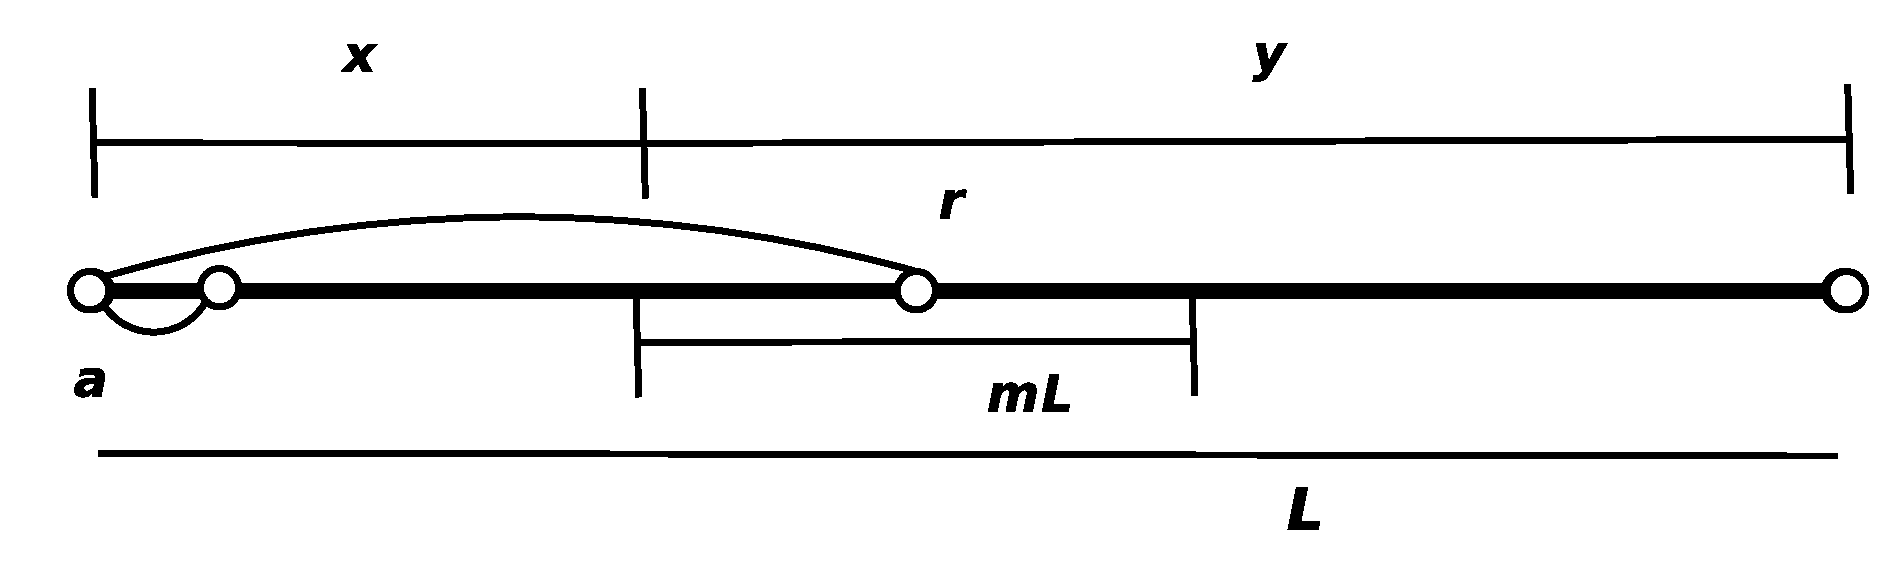
\includegraphics[width=2.5 in]{searchtime}
\caption{The probability that a node \textit{a} has a connection to a node \textit{r} 
in the middle(region \textit{mL}) is defined as $p_{m}$, and $p_m$ is inverse 
proportional to the distance between \textit{a} and \textit{r}.} \label{fig:search}
\end{figure}
From the Kleinberg's model, each node has a long-range
contact at distance \textit{r} with probability 
$p_{r}=\frac{1}{\log N}\frac{1}{r}$ as in Figure \ref{fig:search}. 
Let \textit{$p_{m}$} be the probability that node \textit{a} has a long-range
contact in the middle, \textit{$mL$} region.
\begin{eqnarray*}
p_{m} &=& \sum_{r=\frac{1-m}{2}L}^{\frac{1+m}{2}L}p_{r} = \sum_{r=\frac{1-m}{2}L}^{\frac{1+m}{2}L}\frac{1}{\log
        N}\frac{1}{r}\\
        &\simeq& \frac{1}{\log N}\log\left(\frac{1+m}{1-m}\right)
\end{eqnarray*}
Since \textit{$mL$} is a subset of \textit{$L$},
$m\in (0,1)$. 
Let $T(i)$ be the search time in region of size $i$.
Each long range connection either goes to a node in the
middle region or not.
If we make it into the middle region, the remaining area
to search is at most the length of $\frac{1}{2}L + \frac{m}{2}L$.
Thus,
if the long-range connection goes to the middle, the time is 
$T(L) \leq 1 + T((\frac{1+m}{2})L)$. 
Otherwise, we go to the next neighbor so $T(L) = 1 + T(L-1)$.
We know that $T(L-1) < T(L)$.  
%If $p_m$ is the probability of making it into the middle, on average, 
We need to try $1/p_m$ neighbors before
we are likely to find a connection to the middle.  Putting this together,
the average search time is
$T(L) \leq \frac{1}{p_m} + T((\frac{1+m}{2})L)$. 
The first part of the right side of the equation represents time to reach 
a connection in the middle (\textit{x} in Figure \ref{fig:search}) and 
the second part is time for the rest of the region (\textit{y} in Figure \ref{fig:search}. 
For the rest of the region, at most $\gamma$ more steps are required to 
cover the whole region \textit{L}. We know $T(\log{N}) \leq \log N$. 
Solving for $\gamma$ such that $(\frac{1+m}{2})^{\gamma}L = \log N$, we
find $\gamma \leq \frac{\frac{1}{2}\log{(\alpha N})}{\log{(\frac{1+m}{2})}}$

The maximum depth is decided to $\gamma$ steps multiplied by the number of the nodes 
to reach a connection in the middle.
\begin{eqnarray*}
T(L) &\leq& \frac{1}{p_m}\gamma = \frac{\log N}{\log{(\frac{1+m}{1-m})}}\frac{\frac{1}{2}\log{(\alpha N)}}{\log{(\frac{1+m}{2})}}
 \\
     &\leq& \frac{\frac{1}{2}(\log^2 (\alpha N)-\log{\alpha}\log{(\alpha N))}}{\log{(\frac{1+m}{1-m})}\log{(\frac{1+m}{2})}}
\end{eqnarray*}
At a value of $m\approx0.517$, the denominator of the right side of the above inequality has a minimum. 
In consequence, the upper bound for $T(L)$ is minimized.
We verify this claim using simulations which are presented in Figure \ref{fig:time}. 
%For the comparison, the minimum of upper bound, where \textit{m} is set to 0.5, is 
%calculated and compared with our simulation result.

\subsection{Stabilization Cost}
\label{sec:stabilization_cost}
We regard the number of objects that need to be copied to 
a newly joined node as the stabilization cost ($S$) 
because there is no other major message transmission 
except this copying for a leaving or joining node. 
%We assume that our algorithm checks 
%each object is copied by only one neighbor.
%If a node identifies the 
%object, it discontinues the object transmission. This ensures that a node 
%prevents unnecessary message generation and a network saves bandwidth.
Objects which already exist in a new node as well as out of 
object's range are excluded from transmission.
A new node examines each object's range whenever it is ready to be copied.
In P2P networks, network size often varies. Thus, as the network
size changes, the object's range is recalculated.
Copying in a redefined range constrains the number of 
cached replicas to remain $\sqrt{\alpha N}$.
 
Let $S$ represent the stabilization cost, $k$ be the number of unique objects in the network, 
$N_1$ be the left neighbor, 
and $N_2$ be the right neighbor. Let $\eta_i$ symbolize a probability of the object in node $N_i$. 
$\eta_{ij}$ is a probability of the object in both $N_i$ and $N_j$ and  
$\eta_{j|i}$ denotes a probability of the object in $N_j$ given that the object is in 
$N_i$. 
%\begin{eqnarray*}
%S   &=& k (\eta_1+\eta_2-\eta_{12}) \\
%    &=& k (\eta_1+\eta_2-\eta_1\eta_{2|1})
%\end{eqnarray*}
The probabilities, $\eta_i$ and $\eta_{ij}$, are calculated as follows:
\begin{eqnarray*}
\eta_1 &=& \eta_2 = \frac{L}{B} = \sqrt{\frac{\alpha}{N}} \\
\eta_{12} &=& \eta_1 \eta_{2|1} = \sqrt{\frac{\alpha}{N}}\left( 1-\frac{d_{ave}}{L} \right)
= \sqrt{\frac{\alpha}{N}}\left(1-\frac{1}{\sqrt{\alpha N}}\right) \\
\end{eqnarray*}
The stabilization cost is $\eta_1+\eta_2-\eta_{12}$.
\begin{eqnarray*}
S &=& k\left(2\sqrt{\frac{\alpha}{N}}-\sqrt{\frac{\alpha}{N}}\left(1-\frac{1}{\sqrt{\alpha N}}\right) \right) 
    %&=& k(\sqrt{\frac{\alpha}{N}}+\frac{1}{N}) \\
    = O\left(k\sqrt{\frac{\alpha}{N}}\right)
\end{eqnarray*}
where $d_{ave}$ denotes the average distance between two nodes, 
$N$, $B$, and $L$ represent the number 
of nodes, the ring distance ($d_{ave}N$), 
and the length of bounded broadcasting range ($d_{ave}\sqrt{\alpha N}$), respectively.
%Since $L = \sqrt{\alpha N}d_{ave}$ and $B = d_{ave}N$, 

\section{Simulation Results}\label{sec:simulation}
Our theory results are in terms of $N$, the
size of the network, but local nodes only have estimates of network
size.  We see in this section that following the protocol with network
size estimates based on local node density\cite{LuoQHC08}
does not cause significant deviation from our theory.
%tw: elaborate on the simulator
We developed a C++ simulator for the Deetoo algorithm.
In our topology model, 
each bin may be occupied by at most one node and the nodes form two rings,
one for the cache and the other for query.
%
Each node is connected to a long-range neighbor according
to the \emph{inverse $r^{th}$-power distribution} for the small-world network model. 
For simplicity, the size of the query range is assumed to be the same as the size of the cache 
range. All caching and querying processes are initiated on randomly selected nodes and
messages are broadcasted within randomly chosen ranges.
Network size ($N$) determines the range of bounded broadcasting for both caching and querying, and
success probabilities and communication costs depend on the accuracy of our estimation of $N$.
%The analysis of trade-off between accuracy and cost will be analyzed as future work.

\subsection{Performance Evaluation} 
\begin{figure}
\centering
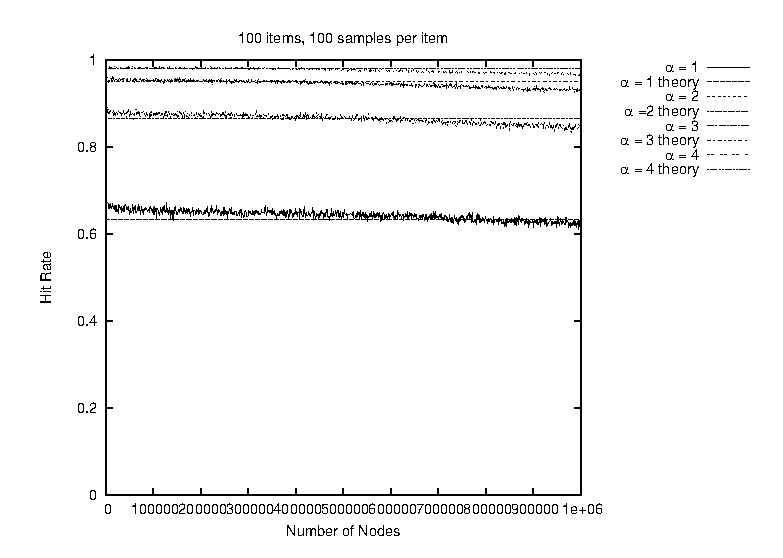
\includegraphics[width=3in]{th_hitrate1}
\caption{Query hit rate is almost constant in network size $N$, and scales
as $1-e^{-\alpha}$. The difference is due to the accuracy of nodes locally 
estimating network size. In the legend, ``th" is theory, the other is simulated.} \label{fig:hitrate}
\end{figure}
%\begin{figure}[h]
%\centering
%\includegraphics[angle=270, width=3.5in]{mishit_logy}
%\caption{Query miss rate as a function of $\alpha$, this scales
%as $\exp(-\alpha)$.} \label{fig:mishit}
%\end{figure}
In our simulations the size of the address space is set to 32 bits which has $2^{32}$
bins. 
We count the number of hops as an indication of communication cost and assume that the 
per-hop communication costs for cache and query are the same. 
Our simulations are performed on networks of size 10 to $10^{6}$.
The number of columns, $C$, is chosen such that $C$ is equal to the number of rows, $Q$, 
$C^2 = \alpha N$. Thus, we simulate various values of $\alpha$ to observe the effect of
increasing or decreasing the cache or query range size ($\alpha=\frac{C^2}{N}$). 
We performed simulations with $\alpha$=0.1 to 5.0, with intermediate steps of size 0.5.
100 string objects were generated by using a random string generator.
%Each object was initially inserted on a uniformly randomly selected
%node.
For queries, we count only exact matching objects even though Deetoo can perform partial matches.
Each test was repeated 100 times and the results were averaged. 
Figure \ref{fig:hitrate} shows that query success probability is almost constant 
regardless of the network size. The difference between the simulation results and 
the theoretical results is due to the accuracy of locally estimated network
size.
The constant success rate is desirable since 
Deetoo can perform the search with preferred success probability by adjusting 
broadcasting range with different $\alpha$.  
In the figure, we also compare the simulation results with the theoretical results.
%We observe that the larger the $\alpha$ is, the higher the success probability is.
%In Figure \ref{fig:mishit}, query success probability declines exponentially as expected.
% POB: we are deleting this because we don't understand it very well. 
%Relatively high deviation is witnessed with large $\alpha$. Because we estimated success
%probability by assuming $\frac{N}{B} \ll$ 1, it is expected to have
%higher deviation in the case where $N\approx B$.
%
%communication cost (hops)
Figure \ref{fig:cost} shows communication cost with respect to network size. There is 
a trade-off between success probability and the communication cost. 
\begin{figure}
\centering
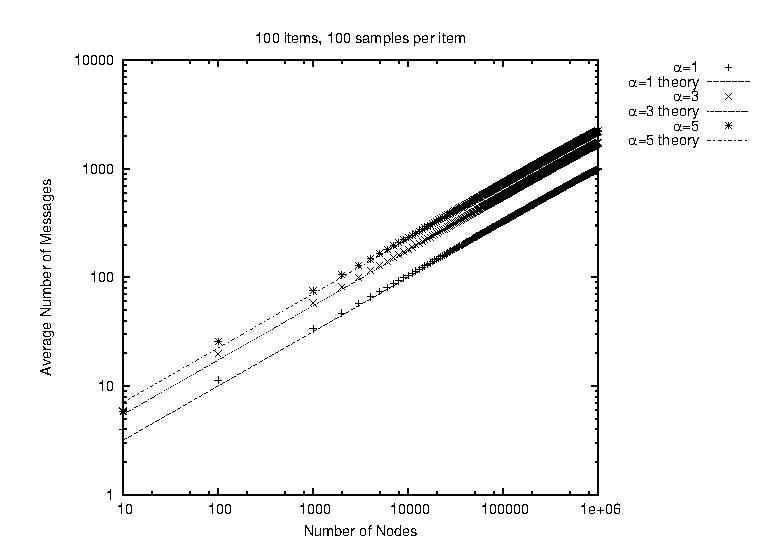
\includegraphics[width=3in]{th_hops_loglog1}
\caption{Query cost scales $O(\sqrt N)$. ''th" is for the theoretical result, 
and the other is the simulation result.} \label{fig:cost}
\end{figure}

%search time (depth)
For the search time, we measured the number of out-of-range links before finding 
a node in the range and the depth of the multicasting tree. 
%Message transmission times at each link are assumed to be all the same. 
Figure \ref{fig:time} %\ref{fig:time5} 
compares simulation results with calculations with $\alpha$=1. 
As mentioned in Section \ref{sec:search_time}, 0.5 is substituted for $m$. 
%Note that \textit{x} axis scales logarithmically. 
Our simulation shows a loose upper bound for search time, 
but it is obvious that the scaling of simulation result is more than 
$\log N$.
%solving  for m as optimal value, 1/2.....
\begin{figure}
\centering
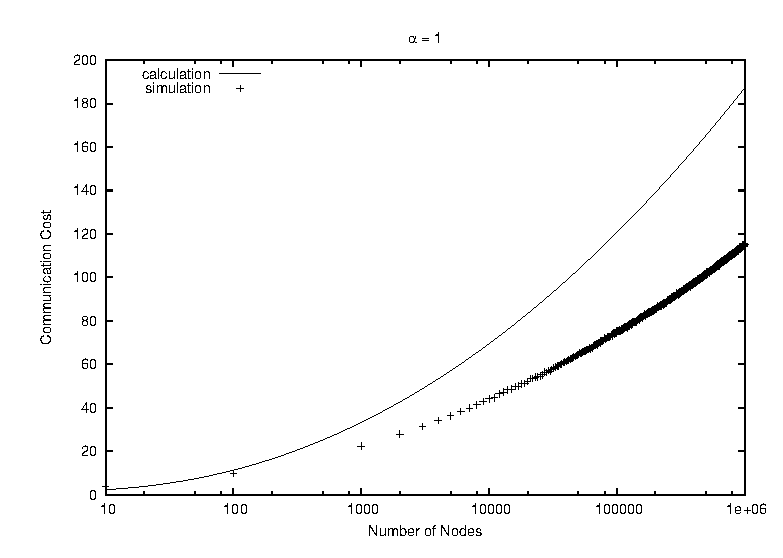
\includegraphics[width=3in]{time1}
\caption{Search time: We see our upper bound is loose, but the search time grows 
more than $\log N$, less than $\log^2 N$.} \label{fig:time}
\end{figure}

\subsection{Robustness}
Due to the nature of P2P networks, each peer can leave or fail 
at any time. Therefore, it is important to analyze the effect of node failures.
We will show that data objects are still accessible without generating 
excessive managing overheads under dynamic networks.
%We extended Netmodeler %\cite{netmodeler} 
%to model massive churn on nodes. 
%The simulator setting is described below.
We set the network size first. Each node joins the network sequentially
following a uniform distribution.
Upon completing network formation with a given size, each node repeatedly 
leaves and joins.
The average number of alive nodes remains half of the nodes initially joined
by setting that each node's rejoin and leave time is exponentially distributed
with same mean.
%ambiguous
%A node's rejoin time and leave time is exponentially distributed with same mean. 
%
%The consequence of this distribution makes the average number of 
%alive nodes in the system remains half of total number of the nodes 
%originally joined. 
%As seen in the Figure \ref{fig:markov}, a 
%A node's state transits between \emph{ON} and \emph{OFF} with probability of 0.5. 
%In other words, 
The probability that each node is active at time t is $\frac{1}{2}$.
%In our simulation setting, every node stays to be turned \emph{ON} until 
%network size reaches a given number. 
%%confusing
%It takes time a network size is saturated at the half of initial network size on average. 
%reason
%\begin{figure}
%\centering
%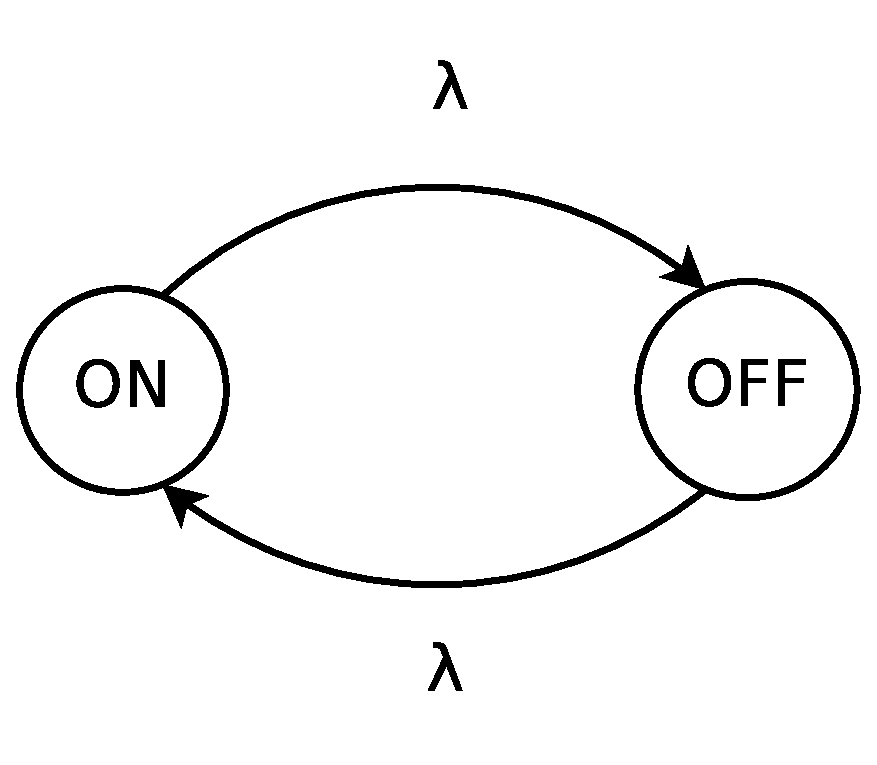
\includegraphics[width=2.5in]{queueingmodel}
%\caption{State Transition Diagram for each node. Because join time and leave time 
%distribution has same average, the probability that each node is alive 
%at a time t is 0.5.} \label{fig:markov}
%\end{figure}
After all nodes joined network, 100 data objects were inserted.
Queries were executed 100 times per data object. 
The cache/query events occur 
in a time distributed exponentially.
For simplicity, a replication factor, $\alpha$, is set to 1.
%for the simulations under churn.

\begin{figure}
\centering
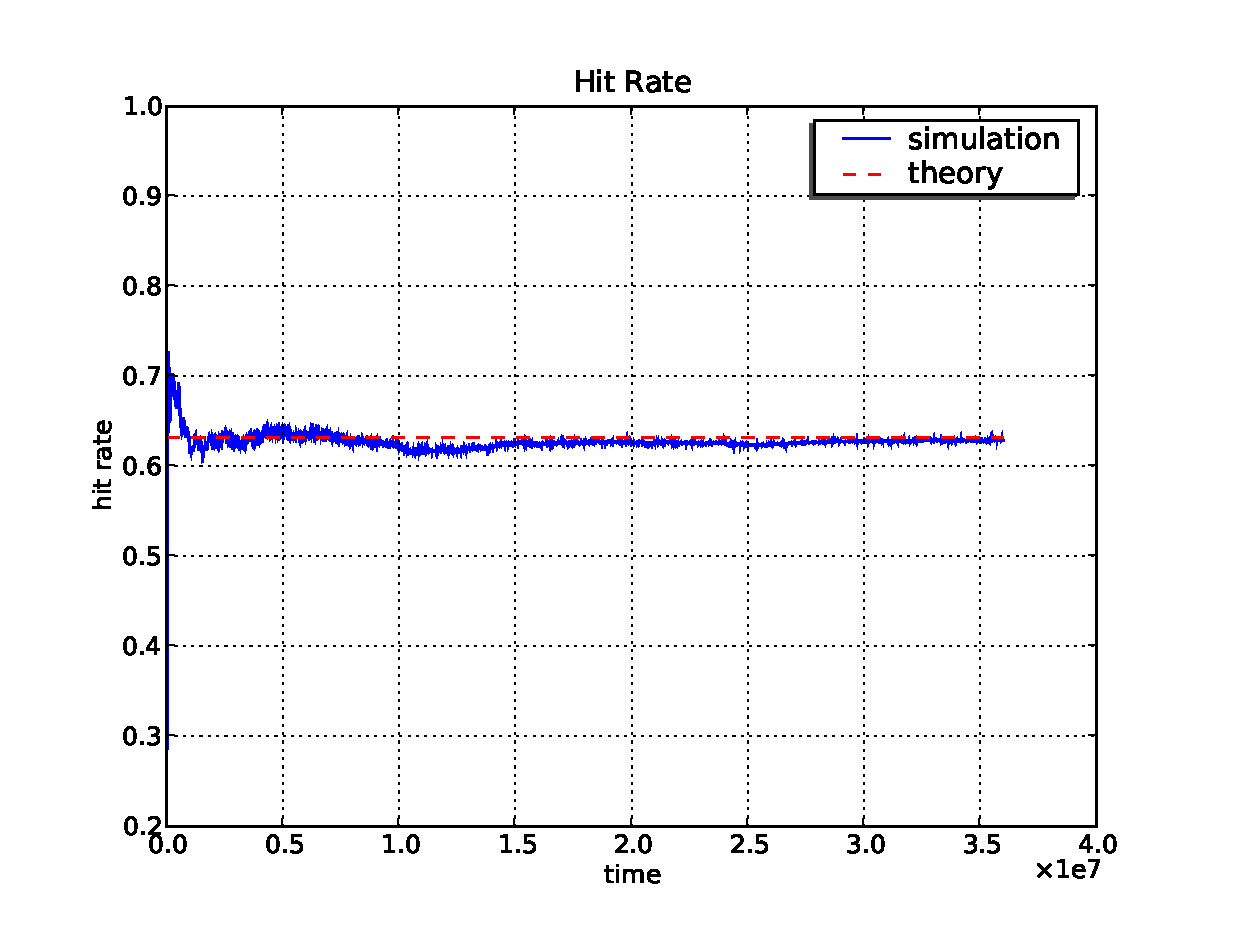
\includegraphics[width=3in]{hit_ch}
\caption{Success probability remains constant under Churn} \label{fig:hit_churn}
\end{figure}
Figure \ref{fig:hit_churn} demonstrates how the churn affects success probability.
Note that success probability remains constant which shows that Deetoo is robust against churn. 
Also, the success probability still follows the theory as described in Section \ref{sec:suc_prob}.
%This result shows that Deetoo is robust against network dynamics. 

\begin{figure}
\centering
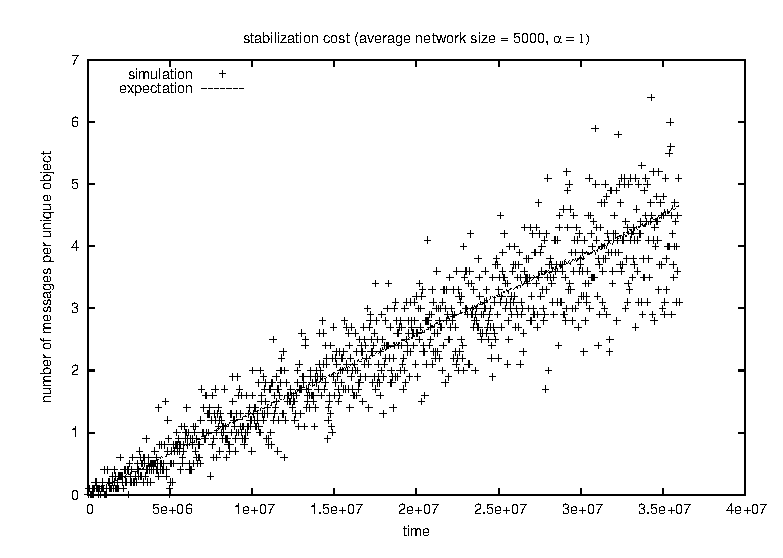
\includegraphics[width=3in]{stab_cost}
\caption{Stabilization Cost} \label{fig:stab_cost}
\end{figure}
Under the heavy churn in the network, message transfers for maintenance purposes
are not negligible. 
%When a new node joins the network, it
%is responsible for maintaining data objects if its address is within 
%objects' range.
We counted what fraction of the total objects were transferred to a new node.
Assume that there are $k$ objects, and each are replicated over 
$\sqrt{N}$ nodes, we have $k$ $\sqrt{N}$ total objects in the system.
%These objects are placed on nodes in the range selected uniformly at random, 
%so 
The expected number of objects on each node is $k/\sqrt{N}$. 
Thus, joining cost is directly proportional to $1/\sqrt{N}$.

Figure \ref{fig:stab_cost} shows that how many replication occurred per unique
data object after new nodes joined. 
For the measure of stabilization cost, 
the size of network is set to 1,000 initially. 
Note that stabilization cost grows not as time continues, but as the number of unique 
objects increases.
Unlike DHT-based stabilization, our process is much simpler, and costs less.
%explain more, what is DHT's cost? compare directly to our cost
With very low maintenance cost, Deetoo is capable of efficient data retrieval 
even under heavy churn.

\section{Related Works}
\label{sec:related_works}
Highly structured P2P networks with DHT look-up algorithms 
\cite{is:Chord, sr:CAN, bz:Tapestry, pr:Symphony} 
are efficient in that these networks achieve low query costs  
because they place data objects at particular points on the network topology
which are determined by an object's key. 
%Beehive\cite{re:beehive04} 
%achieves constant look-up latency on top of a
%DHT through proactive replication. Despite their efficiency, the possibility 
%of operation, even with extremely unreliable nodes, has not been yet
%examined. In addition, 
Generally, it is impossible for them to handle
high-dimensional complex queries.  Extensive research has been conducted 
to address the limits of the exact search problems in DHT.
%more works need to be included (interest-based clustering, distributed kd-tree)
%ex. semantic clustering (SSW)
One example is \emph{pSearch} \cite{psearch}.
In \emph{pSearch}, semantic indices are mapped to a CAN overlay. 
A \emph{rolling index} reduces the number of dimensions for mapping purposes 
onto the overlay and divides the semantic vector(SV) into sub-vectors. 
Each sub-vector has the same number of dimensions as a CAN overlay does.
Although \emph{pSearch} is simple and supports high-dimensional queries, 
it requires control on the data objects of each node. Especially, when 
nodes join and leave frequently, \emph{pSearch} incurs massive overhead.
Therefore, it is more suitable for networks with stable nodes rather than
for highly dynamic networks.
\emph{pSearch} still requires mapping search index into structured P2P overlay, and
this limits the support of general query.
%pSearch only provides best effort search without a bound on accuracy.
\emph{Cubit}\cite{cubit} provides keyword search capability over a DHT. \emph{Cubit} 
efficiently finds multiple closest data sets for a given query. However, 
it requires the creation of a keyword metric space and only returns multiple 
similar results to compensate for typos in queries. 
More complex query resolution methods have been explored for p2p resource 
discovery for grids. \emph{SWORD}\cite{sword}, 
\emph{Mercury}\cite{mercury}, and \emph{MAAN}\cite{maan} 
are proposed to support multi-attribute 
range queries on top of structured overlays.
In \emph{SWORD} and \emph{MAAN}, DHT is created for each attribute.
The number of created DHTs is the same as the number of attributes.
\emph{Mercury} also maintains a logical overlay for each attribute but
it does not use DHTs. These systems can outperforms Deetoo in terms of
query success probability and query cost with the help of DHT. However, 
maintaining multiple overlays costs network traffic
because update traffic increases as the number of attributes are 
increased. Deetoo creates two overlays and update traffic takes 
place only in caching overlay. Moreover, data is not structured,
Deetoo's query is not limited to range query.  

%Deetoo does not demand any keyword mapping 
%into DHT and can execute more general queries like regular expression searches.

%flooding
Unlike DHTs, unstructured P2P systems mostly depend on flooding and random-walking.
The big advantage of unstructured P2P systems 
is the capability of high-dimensional search.
%The early version of Gnutella was based on naive flooding. 
Because flooding produces a very large number of
messages over an entire network, pure flooding limits network size. 
To make unstructured systems scalable, systems such as Gnutella and
Kazaa use supernodes to handle caching and routing query messages.
This work compliments this approach as our algorithm can be employed
by the supernodes to enable a trade-off on query and cache cost that
is not available in existing supernode approaches.
%To address this scaling problem, various types of solutions have been 
%proposed. 
%KaZaa\cite{kazaa} and iXChange
%\cite{JohnstoneSM05} introduced central server-like super-peers. 
%However, super-peers cause bottle-necks, security issues, and the single 
%point of failure problems due to their server-like characteristics. 
Recently, research efforts have also focused on locality-based flooding. Systems 
adopting interest-based locality\cite{Guo05,SMZ03} assume that 
two peers having common interests share pieces of a data object. 
Under this assumption, a shortcut 
connection is established between two peers having common interests, 
and queries from one peer are delivered through this 
shortcut link in the first stage of flooding. 
Locality-based flooding requires warm-up procedures to gather query 
history for shortcut connections. 
\textit{LightFlood}\cite{JiangGZW08} uses a neighbor-degree-based locality scheme. 
\textit{LightFlood} forms a tree-like sub-overlay called 
\textit{FloodNet} using neighbors' degree information. 
%Once the sub-overlay 
%is formed, there are two overlay networks in the system: the original 
%P2P overlay and \textit{FloodNet}. 
The flooding takes two stages.
Messages are transmitted using pure flooding with relatively small TTL values 
in the first stage. The peers that receive the query with zero TTL trigger 
the second stage of flooding in the \textit{FloodNet}. Although 
\textit{LightFlood} is simple and helps stop generating massive messages 
for queries at a certain point, searching unpopular objects requires  
the entire network to be visited; in addition, \textit{LightFlood} needs to 
be warmed up to form sub-overlay.  
A random walk based search technique is introduced by Adamic et. al. 
in \cite{alph:powerlaw01} to reduce search cost by the factor of 
the number of replicas, but they do not consider replica placement. 
Although random walk search has an advantage over flooding
in terms of search cost, it has some
scalability problems because almost all the queries tend to concentrate
on the high degree nodes. To address this problem, object
replication with square-root principle\cite{CohenS02,LCKS02}
and topology reconstruction\cite{Cooper05} have been proposed. 
Both reduce search time but incur considerable communication cost 
to maintain fresh topologies or data replication copies. 
%Popularity-biased random walk\cite{zs:popularity06}
%achieves square-root principle without the cost of data movement or
%topology reconstruction. 
Sarshar et al. \cite{ns:percolation}
combined flooding and random walking in power-law networks. In their
work, a query can be resolved in time $O(\log N)$. However
$O(N\times \frac{2log k_{max}}{k_{max}})$ messages are
transmitted for a single query, where $k_{max}$ denotes the maximum
degree; thus, when $k_{max} = \sqrt{N}$ this becomes $O(\sqrt N \log N)$.

Liu et al. \cite{LiuHZ04} study bounded broadcasting in wireless sensor networks. 
A balanced push and pull strategy achieves $O(\sqrt N)$ search 
cost in the best scenario. However, the \emph{comb-needle data discovery}  
requires to estimate cache and query frequency.
All nodes should keep their location information in the grid. 
Though they do not analyze search time, it is possible to estimate it. By the
nature of the hop-by-hop message transfer, the \emph{comb-needle data discovery} 
takes linear time in the bounded range which is $O(\sqrt N)$. 
The \emph{dynamic paths} quorum system\cite{Naor05} 
is scalable and operates in a dynamic setting. The quorum sets are 
divided into reading quorums and writing quorums in a grid, and each 
reading quorum intersects each writing quorum. Naor et al. analyzed probe 
complexity and availability, especially in a dynamic environment. 
The probe complexities of the non-adaptive (without stabilization)
and adaptive (with stabilization) algorithms is 
$\Theta(\sqrt N \log N)$ and $\Theta(\sqrt N)$, respectively. 



\section{Conclusion and Future Work}
\label{sec:conclusion}
In this paper, we introduced Deetoo, a scalable unstructured searching
algorithm for unstructured P2P networks which provides efficient caching
and lookup functionality with a constant query hit-rate, $O(\sqrt N)$
replication, $O(\sqrt{N})$ query cost, and $O(\log^2 N)$ search time.

Deetoo, allows objects to be updated and deleted, and can
be used to handle general queries.  Specifically, any problem
that can be mapped onto selecting (with high probability) objects
which match some query can be run over Deetoo.

In our future work, we plan to implement this searching algorithm
on Planet-Lab nodes and to compare the performance of Deetoo with
existing search schemes. Additionally, due to the
fact that Deetoo is already a randomized algorithm, we are
investigating optimal approaches for dealing with lossy communications
such UDP/IP datagrams which go beyond naive hop-by-hop retransmission.

\bibliographystyle{IEEEtran}
\bibliography{d2}

\end{document}
